\documentclass[12pt,a4paper]{article}

\usepackage[utf8]{inputenc}
\usepackage[greek,english]{babel}
\usepackage{alphabeta}

\usepackage[pdftex]{graphicx}
\usepackage[top=1in, bottom=1in, left=1in, right=1in]{geometry}

\linespread{1.06}
\setlength{\parskip}{8pt plus2pt minus2pt}

\widowpenalty 10000
\clubpenalty 10000

\newcommand{\eat}[1]{}
\newcommand{\HRule}{\rule{\linewidth}{0.5mm}}

\usepackage[official]{eurosym}
\usepackage{enumitem}
\setlist{nolistsep,noitemsep}
\usepackage[hidelinks]{hyperref}
\usepackage{cite}

% --- added packages ---
\usepackage{amsmath,amssymb}
\usepackage{booktabs}
\usepackage{tabularx}
\usepackage{xcolor}
\usepackage{tikz}
\usetikzlibrary{arrows.meta,decorations.pathreplacing}

% Figures are generated into ../figures by scripts/make_report_figures.py; the tables in
% tables/ are generated by scripts/write_report_tables.py from reports/tables/*.csv.
\graphicspath{{../figures/}}

% Red marks content we are not confident about or that still needs a decision or a check.
% Search for \tbc to find every such place. Delete the markers before submission.
\newcommand{\tbc}[1]{\textcolor{red}{[#1]}}


\begin{document}

	%===========================================================
	\begin{titlepage}
		\begin{center}

			\includegraphics[width=0.55\textwidth]{the-university-of-sydney-vector-logo.png}~\\[2cm]

			\HRule \\[0.4cm]
			{ \LARGE
				\textbf{Project Report for ENGG2112}\\[0.4cm]
				\emph{Early Warning of Fault and Downtime Episodes in Wind Turbines using SCADA Data from the Hill of Towie Wind Farm}\\[0.4cm]
			}
			\HRule \\[1.5cm]

			{ \large
				\tbc{Kanav Veer Singh, 550767295, Software Engineering} \\[0.1cm]
				\tbc{Name, SID, Discipline} \\[0.1cm]
				\tbc{Name, SID, Discipline} \\[0.1cm]
				\tbc{Name, SID, Discipline} \\[0.1cm]
			}

			\vfill

			\textsc{\large Faculty of Engineering}\\[0.4cm]

			{\large \today}

		\end{center}
	\end{titlepage}

	\begin{center}
	\subsection*{Executive Summary}
	\end{center}

	\noindent Unplanned stops of wind turbines are expensive: they halt energy production, often need a crew and parts at short notice, and are usually noticed only after the turbine has already stopped. This project asks whether the data a turbine already records every ten minutes can warn of a coming fault or long stoppage in time to plan around it, and whether such a warning can be explained well enough for a maintenance engineer to trust it.

	We used the open Hill of Towie dataset (21 Siemens SWT-2.3-VS-82 turbines in Scotland, January 2016 to April 2026). Because the alarm log contains many routine events, we defined a failure as a \emph{fault episode}, in two related ways: days with at least four hours of recorded fault time (target A), and at least three hours with the rotor stopped despite enough wind (target B). For every turbine-day we predicted whether a new episode would start in the next 30 days. We compared simple rules, a normal-behaviour model, logistic regression and class-weighted gradient boosting (LightGBM), trained on 2016--2018 and 2020, tuned on 2021--2022 and tested once on 2023 to April 2026. Because about half of all days are positive, we always compared each model with a random score.

	Our main finding is a cautious one. \textbf{On the test years no model could be distinguished from the random score}: every 95\% interval for the area under the precision--recall curve (PR-AUC) contains the random-score value. The learned models (LightGBM, logistic regression) had the highest point estimates, about 0.04 above the best simple rule, but the intervals overlap. The model that looked best on the tuning years (a per-turbine z-score of temperatures) fell back to the random level on the test years, and the alert threshold chosen on the tuning years did not hold a fixed false-alarm rate. A model of the normal behaviour of the turbine temperatures gave a weak health indicator that drifts between years. The explanations were stable across turbines but describe a model with no demonstrated skill.

	Because the result was weak, we ran four further pre-registered rounds on the tuning years only, leaving the frozen results untouched: drift-robust features, each turbine's own recent history as baseline, pruning the least useful of about 250 inputs, and 27 alternative definitions of the label. Roughly 390 configurations were evaluated. None moved the learned models beyond the random-score margin of error; pruning showed that 50 to 100 inputs do as well as all of them; and one simple baseline, a rotor-speed-against-wind-speed curve, ranked turbines better than chance on the tuning years under almost every label definition. That is a lead to check on fresh data, not a result. We therefore do not recommend deploying any of these models. The shortcomings that limit what this study can show are collected in Section~\ref{sec:limits}, and the next steps, led by obtaining confirmed failure records, are in Section~\ref{sec:disc}.

	\newpage

	%===========================================================
	\tableofcontents
	\addtocontents{toc}{\protect\thispagestyle{empty}}
	\newpage
	\setcounter{page}{1}

	%===========================================================
	\section{Background and Motivation}\label{sec:intro}

	Operation and maintenance (O\&M) typically accounts for 20--25\% of the levelised cost of energy (LCOE) of wind power, and 11--30\% for onshore projects \cite{irena2012}. Much of this comes from \emph{unscheduled} maintenance, where a component fails without warning and the turbine stays idle until technicians and parts arrive \cite{carroll2016}. Shifting from reactive or fixed-interval maintenance to \emph{predictive} maintenance, intervening when the data indicate that a failure is approaching, is one of the most direct ways to reduce this cost.

	Every utility-scale turbine already logs data through its \emph{Supervisory Control and Data Acquisition} (SCADA) system, typically as 10-minute statistics of power, speeds, wind, pitch and dozens of component temperatures, plus an alarm log. SCADA-based monitoring therefore needs no extra sensors, unlike dedicated vibration-based systems that are costly to retrofit \cite{tautzweinert2017}. Yet alarms are used almost entirely \emph{reactively}, and large farms can raise so many that operators struggle to interpret them \cite{qiu2012}. Many alarms are also routine: in our data three alarm codes are present in more than 99\% of 30-day windows (Figure~\ref{fig:alarmrates}), so ``an alarm fired'' is a poor definition of ``something is wrong''. This is why we define the failures to predict from recorded fault time and rotor stops (Section~\ref{sec:prob}) and use alarm counts only as inputs.

	We use the \textbf{Hill of Towie open dataset}, released by RES on behalf of TRIG under CC-BY-4.0 \cite{hot_dataset_v1,hot_dataset_v2}: 21 Siemens SWT-2.3-VS-82 turbines at a commercial wind farm in Scotland, with 10-minute SCADA statistics and the alarm log from January 2016 to April 2026 (version v2.1.0 \tbc{version still to be confirmed with the person who downloaded the data; the brief cited v1.0.0, which ends earlier}). We used five tables: three 10-minute SCADA tables (temperatures, pressures and the main turbine signals), the alarm log and a daily summary that includes the recorded fault time. The data dictionary lists further tables, for active power and for error time, which were not in our files, so we used proxies (Section~\ref{sec:meth}). The temperature and pressure tables for 2019 are missing from our copy, so 2019 is not used. \tbc{The number of temperature fields (27 in the earlier draft) and the statement that the publishers list alarm prediction as an intended use, while the released example analyses focus on energy yield and upgrade uplift \cite{res_repo}, still need to be checked against the data dictionary and the record page.}

	\section{Objectives and Problem Statement}\label{sec:prob}

	The \textbf{primary objective} is to predict, using only standard 10-minute SCADA data and the alarm log, whether a turbine will enter a fault or downtime episode in the near future, and to be honest about how much better than chance this is. The four objectives are to:
	\begin{enumerate}[label=\textbf{O\arabic*}]
		\item build a degradation indicator: a model of normal behaviour whose gap to the observed temperatures is a health score;
		\item predict fault and downtime episodes within 30 days with models of increasing complexity, and compare each with a random score on the false-alarm budget of one per turbine-month;
		\item test robustness: to a turbine unseen in training, to missing sensor groups, and across years;
		\item explain the predictions, as attribution to model inputs and not as proof of cause.
	\end{enumerate}

	\paragraph{Targets.} The alarm log contains many routine events, so alarm codes are not the target. Target A marks a usable day as a \emph{fault day} when the recorded fault time (\texttt{TimeErr} in the daily summary) is at least four hours; target B marks a \emph{stop} when the generator speed is below 200\,rpm for at least 18 consecutive 10-minute intervals (three hours) while the primary wind speed is at least 4\,m/s. In both, fault days or stops separated by fewer than seven fault-free days form one \emph{episode}. The meaning of \texttt{TimeErr} is not documented by the data provider; we infer it from its name and from its agreement with the SCADA stop time (correlation 0.86), so ``fault'' here means ``recorded fault time'' and not ``confirmed component failure''. The two targets are related cross-checks, not independent confirmations: about three quarters of the episodes of one have an episode of the other starting within seven days (Figure~\ref{fig:agreement}).

	\paragraph{Formal statement.} Let $k \in \{1,\ldots,21\}$ index turbines and $d$ index turbine-days, with $\mathbf{x}_{k,d}$ the features of day $d$ built from data up to the end of that day only. The model input is the \emph{observation window} of the last $W=7$ days, summarised into window means and standard deviations. For the \emph{prediction horizon} $H=30$ days, the label is
	\begin{equation}
		y_{k,d} =
		\begin{cases}
			1 & \text{if an episode starts on turbine } k \text{ in } (d,\, d+H], \\
			0 & \text{otherwise.}
		\end{cases}
	\end{equation}
	Rows that cannot be labelled honestly carry no label and are not used for training or scoring: days inside an episode, days whose next episode starts 30 to 60 days ahead (the \emph{exclusion zone}, because the label there is ambiguous), days whose horizon reaches into another data split, and poorly observed days (Figure~\ref{fig:timeline}). We learn a score $f(\mathbf{x}_{k,d})$ and raise an alert when it exceeds a threshold $\tau$ chosen on the validation years so that the false alarms stay at one per turbine-month.

	\begin{figure}[htbp]
	\centering
	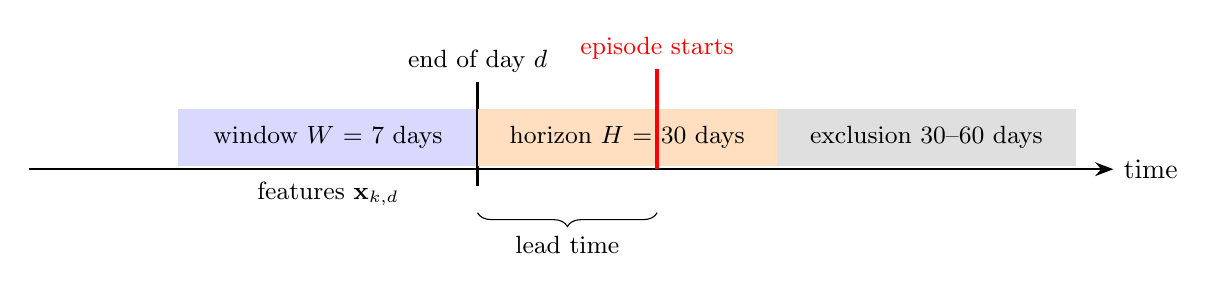
\begin{tikzpicture}[x=0.95cm,y=0.85cm,>=Stealth]
		\draw[->, thick] (0,0) -- (14.5,0) node[right] {time};
		\fill[blue!15] (2,0.05) rectangle (6,0.9);
		\node at (4,0.48) {\small window $W$ = 7 days};
		\node[below] at (4,-0.05) {\small features $\mathbf{x}_{k,d}$};
		\draw[thick] (6,-0.25) -- (6,1.3);
		\node[above] at (6,1.3) {\small end of day $d$};
		\fill[orange!25] (6,0.05) rectangle (10,0.9);
		\node at (8,0.48) {\small horizon $H$ = 30 days};
		\fill[gray!25] (10,0.05) rectangle (14,0.9);
		\node at (12,0.48) {\small exclusion 30--60 days};
		\draw[red, very thick] (8.4,0) -- (8.4,1.5);
		\node[red, above] at (8.4,1.5) {\small episode starts};
		\draw[decorate, decoration={brace, amplitude=5pt, mirror}] (6,-0.65) -- (8.4,-0.65)
			node[midway, below=5pt] {\small lead time};
	\end{tikzpicture}
	\caption{Problem set-up: an episode starts inside the horizon, so $y_{k,d}=1$. An episode that starts in the exclusion zone leaves the day unlabelled.}
	\label{fig:timeline}
	\end{figure}

	\paragraph{Why metrics need care.} Data are split chronologically, since neighbouring days are strongly correlated and a random split would leak the future. Because about half of the labelled days are positive after the exclusions (Table~\ref{tab:labels}), accuracy is uninformative, and so is recall at a fixed number of false alarms: a random score alone reaches episode recall of 0.76 to 0.84 at the budget. We therefore report the area under the precision--recall curve (PR-AUC) against the random-score value, episode recall next to the random-score recall, the median lead time and the false alarms per turbine-month, with 95\% intervals that resample whole turbines (Section~\ref{sec:evalenv}). We do not report precision.

	\section{Related Work}

	\tbc{The citations in this section and in the Background come from the earlier draft and have not been re-checked against the sources; the project rule is to cite only sources that have been verified. Check each statement and each number below against its source before submission.}

	Tautz-Weinert and Watson \cite{tautzweinert2017} group SCADA-based condition monitoring into trending, clustering, normal behaviour modelling, damage modelling, and alarm/expert-system assessment; our work combines the last two by using alarms as inputs to a model of SCADA behaviour and by building a normal-behaviour indicator. Qiu et al.\ \cite{qiu2012} first analysed SCADA alarms directly, showing that alarm volumes overwhelm operators and that alarm sequences carry diagnostic and prognostic information. Leahy et al.\ \cite{leahy2018} trained support vector machines on SCADA data from one Irish turbine, with recall generally above 80\% and fault prediction up to 24\,h ahead. Shah and Tan \cite{shah2025} forecast alarm time series with an LSTM for 14 Senvion MM82 turbines; accuracy fell from 82\% at a 10-minute horizon to 41\% at 30 minutes, which shows the horizon trade-off that we only examined through label variants (Section~\ref{sec:labelsens}).

	Closest to our normal-behaviour indicator, Barrera and Vidal \cite{barrera2026} detect generator faults from SCADA data alone at an eight-turbine farm with one winding-overheating failure. They model healthy phase temperatures using Gramian angular field images and CNNs, flag faults as deviations, fine-tune a global model per turbine (MAE 2.016 $\rightarrow$ 1.479) and use integrated gradients to explain predictions. G\"uck et al.\ \cite{gueck2024} released the CARE benchmark (36 turbines, three farms) with a score rewarding earliness and penalising false alarm events, which informs our metrics and our future work.

	Unlike these studies (Table~\ref{tab:related}), we (i) use openly licensed data so results are reproducible, (ii) define the target as fault and downtime episodes, with two related definitions, over 21 turbines and about ten years, and (iii) evaluate every model against a random-score floor, with intervals that resample turbines, score the test years once, and report the exploratory attempts to improve the result together with how many were tried.

	\begin{table}[htbp]
	\centering
	\small
	\begin{tabularx}{\linewidth}{@{}lXXl@{}}
	\toprule
	\textbf{Study} & \textbf{Data} & \textbf{Method} & \textbf{Horizon} \\
	\midrule
	Leahy et al.\ \cite{leahy2018} & 1 turbine, Ireland & SVM fault classification & up to 24 h \\
	Shah \& Tan \cite{shah2025} & 14 Senvion MM82 & LSTM alarm forecasting & 10--30 min \\
	Barrera \& Vidal \cite{barrera2026} & 8 turbines, 1 generator fault & GAF + CNN normal behaviour model & early detection \\
	\textbf{This project} & 21 SWT-2.3, Hill of Towie & rules, normal-behaviour model, logistic regression, LightGBM & 30 days \\
	\bottomrule
	\end{tabularx}
	\caption{Summary of closely related work.}
	\label{tab:related}
	\end{table}

	%===========================================================
	\section{Methodology}\label{sec:meth}

	\subsection{Study Design and Safeguards}\label{sec:design}
	The study is a pipeline (Figure~\ref{fig:pipeline}) with one rule above all: \emph{nothing fitted, chosen or tuned may use data from a later split}. Raw tables are cleaned, turned into labels and features, fed to models, and evaluated against a random score. Years are split chronologically into training (2016--2018 and 2020; 2019 is unavailable), validation (2021--2022) and test (2023 to April 2026) years. Everything that is learned, including the columns kept, the imputation, the scaling, the normal-behaviour models and the positive-class weight, comes from labelled training rows. Settings and alert thresholds are chosen on the validation years. The test years are scored once, for configurations frozen beforehand.

	The following safeguards are part of the method and are what let us trust the weak result.
	\begin{itemize}
		\item \textbf{One configuration file and a decision log.} Every window, year, budget and seed is in a single file; every decision is recorded with an identifier (D-001 to D-068) on the day it is made, and the configuration is only changed together with its entry.
		\item \textbf{Leakage tests.} A test recomputes random feature rows after deleting everything after the end of their day and checks that no feature changes; the normal-behaviour residuals have the same check; every baseline must pass a score-contract test (a score may not use labels or other rows of the batch).
		\item \textbf{Unlabelled rows stay unused.} Days inside an episode, in the 30--60-day exclusion zone, purged at a split boundary, censored or poorly observed carry no label and enter neither training nor scoring metrics.
		\item \textbf{Pre-registration for exploration.} Each follow-up round (Section~\ref{sec:explmeth}) was written into the decision log, with its configuration grid, before it was run, and reports every configuration, not only the best.
		\item \textbf{A random-score floor everywhere.} Every table or figure shows the random-score value for the same split, target and label definition.
	\end{itemize}

	\begin{figure}[htbp]
	\centering
	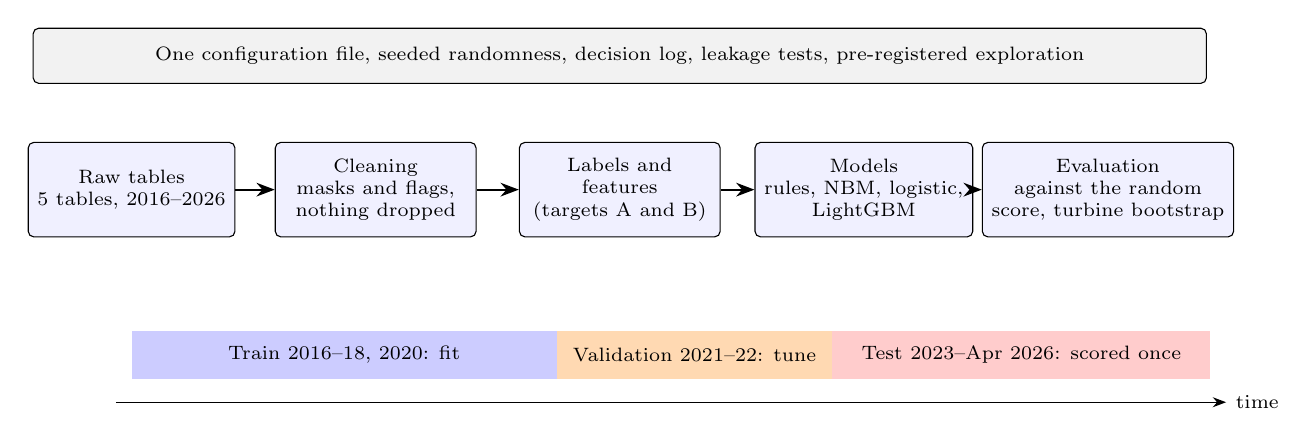
\begin{tikzpicture}[>=Stealth, box/.style={draw, rounded corners=2pt, minimum width=2.55cm, minimum height=1.2cm, align=center, font=\scriptsize, fill=blue!6}]
		\node[box] (raw) at (0,0) {Raw tables\\5 tables, 2016--2026};
		\node[box] (clean) at (3.1,0) {Cleaning\\masks and flags,\\nothing dropped};
		\node[box] (lf) at (6.2,0) {Labels and\\features\\(targets A and B)};
		\node[box] (mod) at (9.3,0) {Models\\rules, NBM, logistic,\\LightGBM};
		\node[box] (ev) at (12.4,0) {Evaluation\\against the random\\score, turbine bootstrap};
		\foreach \a/\b in {raw/clean, clean/lf, lf/mod, mod/ev} {\draw[->, thick] (\a) -- (\b);}
		\node[draw, rounded corners=2pt, fill=gray!10, font=\scriptsize, minimum width=14.9cm, minimum height=0.7cm] at (6.2,1.7)
			{One configuration file, seeded randomness, decision log, leakage tests, pre-registered exploration};
		\fill[blue!20] (0,-2.4) rectangle (5.4,-1.8);
		\node[font=\scriptsize] at (2.7,-2.1) {Train 2016--18, 2020: fit};
		\fill[orange!30] (5.4,-2.4) rectangle (8.9,-1.8);
		\node[font=\scriptsize] at (7.15,-2.1) {Validation 2021--22: tune};
		\fill[red!20] (8.9,-2.4) rectangle (13.7,-1.8);
		\node[font=\scriptsize] at (11.3,-2.1) {Test 2023--Apr 2026: scored once};
		\draw[->] (-0.2,-2.7) -- (13.9,-2.7) node[right, font=\scriptsize] {time};
	\end{tikzpicture}
	\caption{Study design: the pipeline (top) and the chronological split (bottom). Each stage reads only what the earlier stages and the earlier years provide.}
	\label{fig:pipeline}
	\end{figure}

	\subsection{Data Pre-Processing}
	We built every table from the raw monthly files (590 CSV files, 2016 to April 2026). The three 10-minute SCADA tables were de-duplicated (about 2{,}100 duplicate turbine-timestamp keys per table arise at month boundaries), sentinel values were masked to missing per table (for example 200 and $-50$ in the temperature tables, where they mean ``no reading''; 200 is a real value for yaw and nacelle position and is not masked), and the tables were joined on turbine and timestamp, giving 10.14 million rows. The timestamp is the end of the interval (UTC), so a day holds the intervals whose start lies in it, and alarms are joined by rounding up to the next 10 minutes. Nothing was silently dropped: rows keep flags for outage months (2022-08, 2022-09 and 2025-09 have far less than the full set of intervals), for turbine-years whose wind sensor is suspect (four turbine-years), and for the number of masked values (Figure~\ref{fig:coverage}). Active power and error time were not available, so we used generator speed against wind speed instead of a power curve, and \texttt{TimeErr} from the daily summary for target A. Alarm events come from the raw alarm log and not from the processed workbooks, which keep about 0.2\% of the alarms. Several data surprises shaped later choices: sensors that exist only in some years, drifting sensor levels, a change in alarm counts in 2022, and one turbine that is almost always positive (Section~\ref{sec:limits}).

	\begin{figure}[htbp]
	\centering
	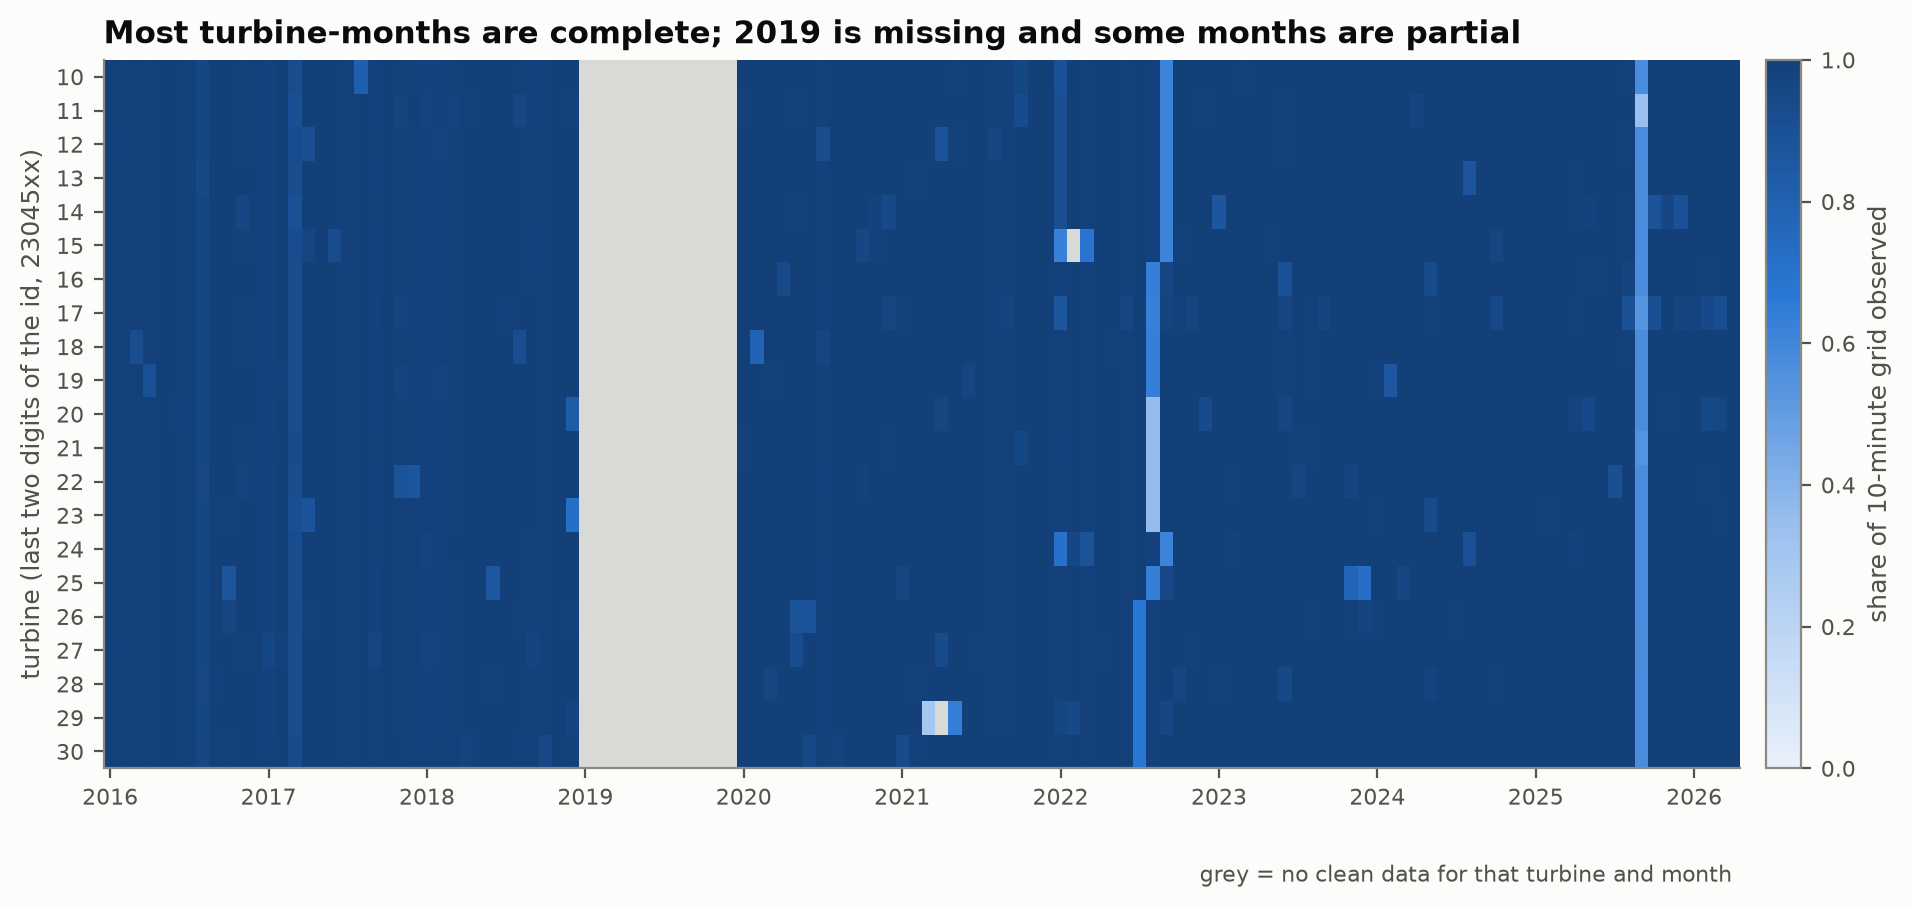
\includegraphics[width=0.85\linewidth]{01_data/F01_coverage_turbine_month.png}
	\caption{Share of the full 10-minute grid observed per turbine and month (F01). Months below 0.9 are flagged as outage months; 2019 is missing.}
	\label{fig:coverage}
	\end{figure}

	\subsection{Targets and Labels}\label{sec:labelsmeth}
	Labels were generated as in Section~\ref{sec:prob} from episodes of each target, with day-resolution episode boundaries. Figure~\ref{fig:alarmrates} shows why alarm codes were not used as targets, and Figure~\ref{fig:agreement} shows how closely the two targets agree. Table~\ref{tab:labels} gives the number of labelled days, positive days and episodes by target and split, and Figure~\ref{fig:labelstatus} shows which candidate days are dropped and why. The positive share is high and uneven across years and turbines (Figure~\ref{fig:positive}), which sets the random-score floor that every model has to beat.

	\begin{figure}[htbp]
	\centering
	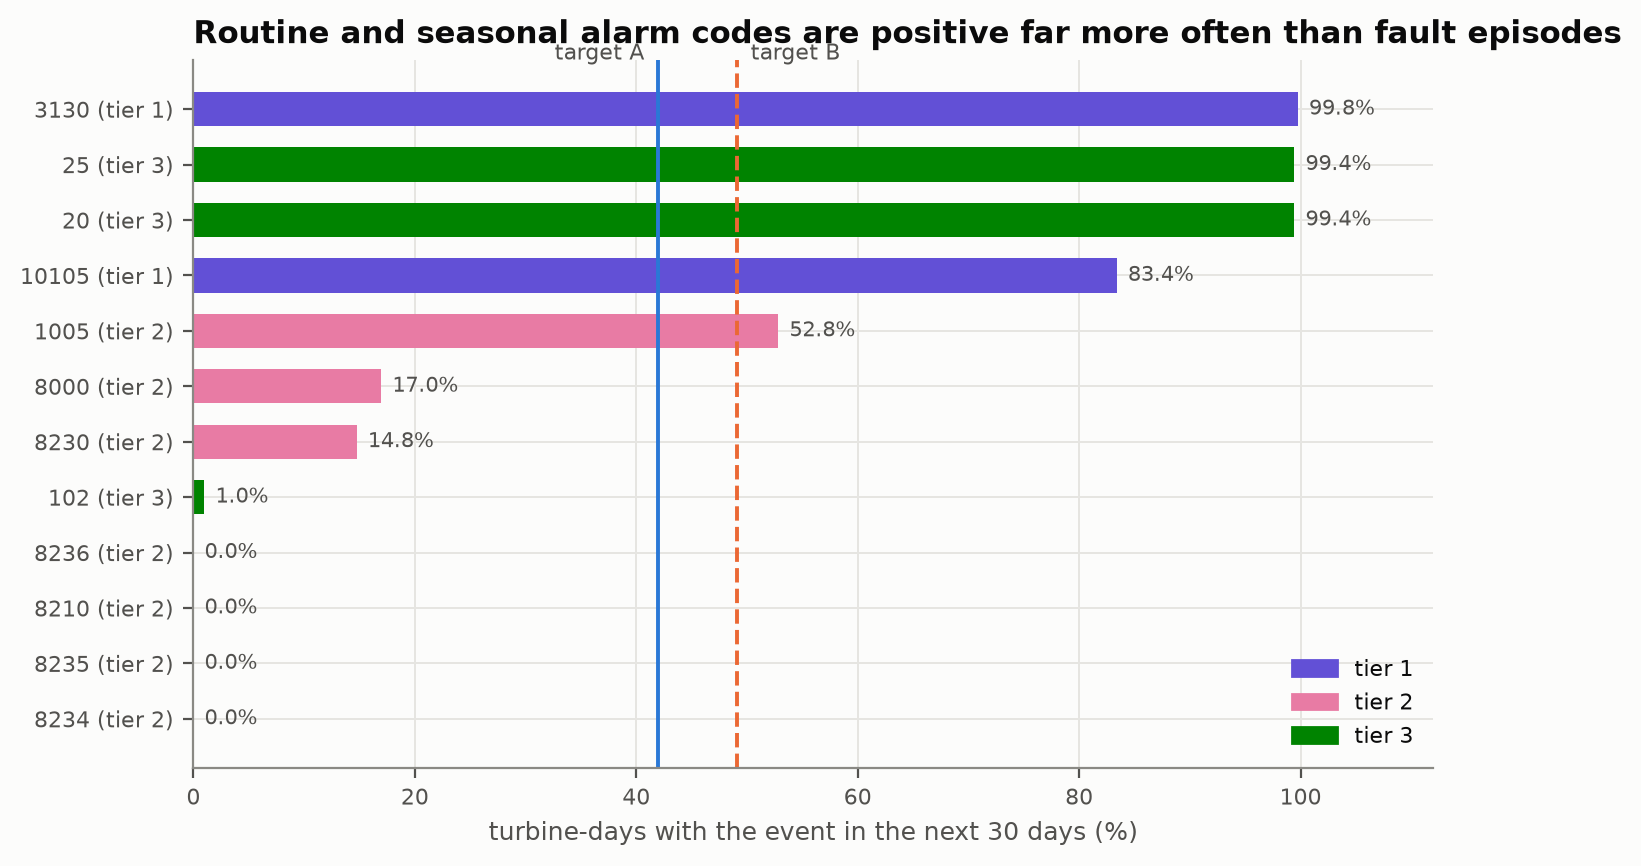
\includegraphics[width=0.9\linewidth]{01_data/F03_alarm_window_rates.png}
	\caption{Share of 30-day windows containing each alarm code, against the share positive for the two targets (F03). Several codes are present almost always, so predicting them would be trivial.}
	\label{fig:alarmrates}
	\end{figure}

	\begin{figure}[htbp]
	\centering
	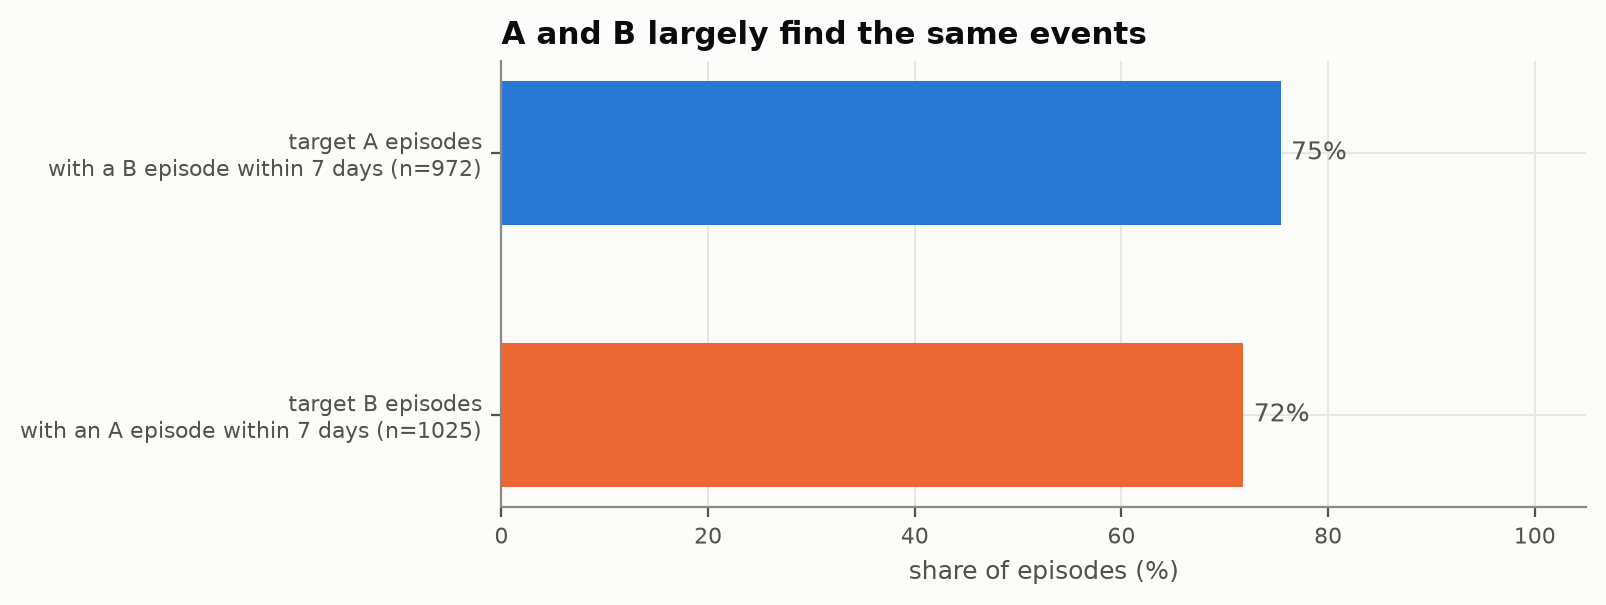
\includegraphics[width=0.85\linewidth]{02_labels/F07_target_agreement.png}
	\caption{Do the two definitions find the same events? (F07) Most episodes of one target have an episode of the other starting within seven days, so A and B are related checks and not independent evidence.}
	\label{fig:agreement}
	\end{figure}

	\begin{table}[htbp]
	\centering
	\small
	\begin{tabular}{@{}llrrrr@{}}
\toprule
Target & Split & Labelled days & Positive days & Positive share & Episodes \\
\midrule
A & train & 22{,}309 & 8{,}315 & 37.3\% & 355 \\
A & val & 9{,}690 & 4{,}558 & 47.0\% & 217 \\
A & test & 17{,}951 & 8{,}099 & 45.1\% & 336 \\
B & train & 20{,}911 & 10{,}001 & 47.8\% & 434 \\
B & val & 8{,}827 & 4{,}346 & 49.2\% & 209 \\
B & test & 17{,}281 & 8{,}725 & 50.5\% & 382 \\
\bottomrule
\end{tabular}

	\caption{Labelled days, positive days and episodes by target and split (\texttt{reports/tables/label\_summary.csv}). Episodes are counted over the whole split.}
	\label{tab:labels}
	\end{table}

	\begin{figure}[htbp]
	\centering
	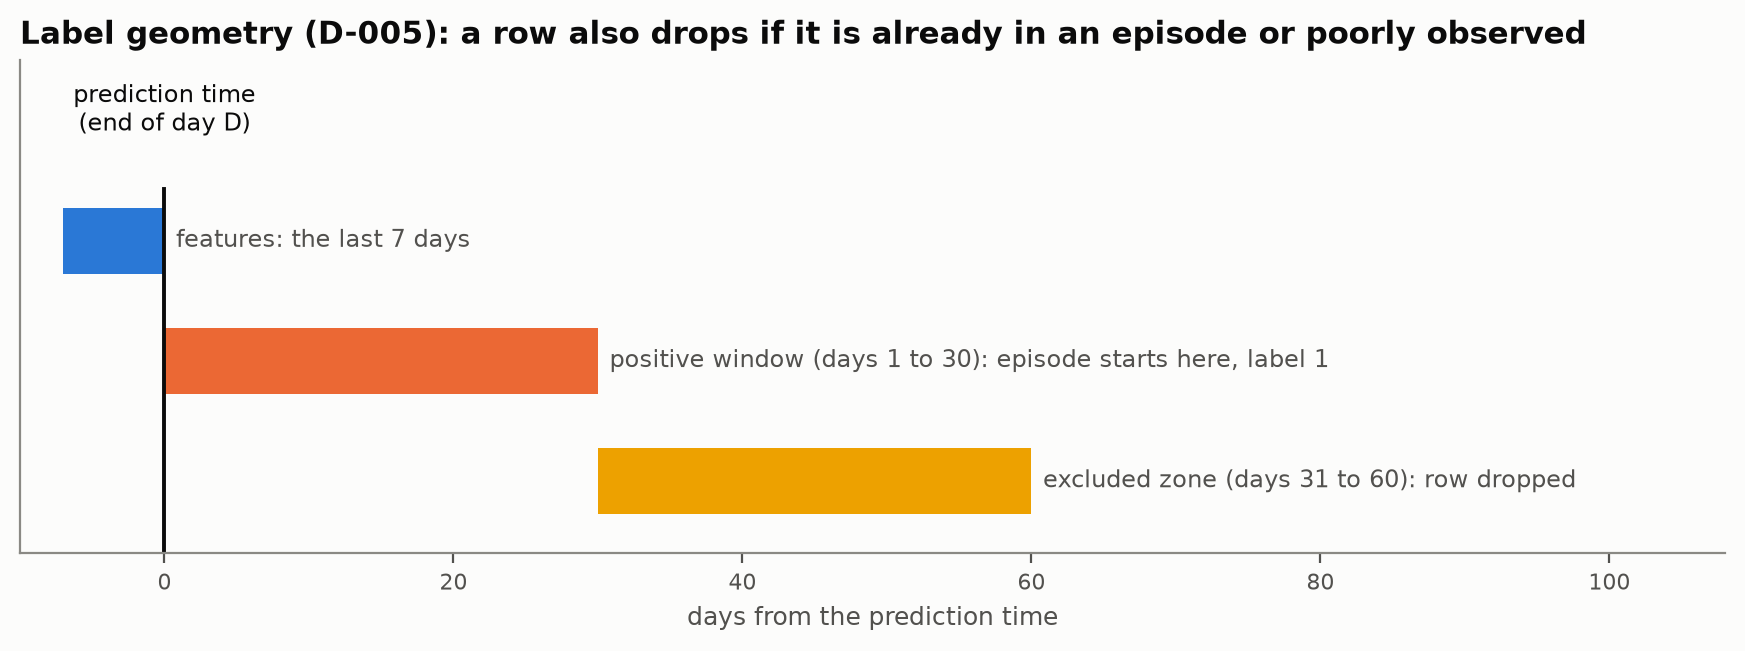
\includegraphics[width=0.8\linewidth]{02_labels/F08_label_geometry.png}\\[4pt]
	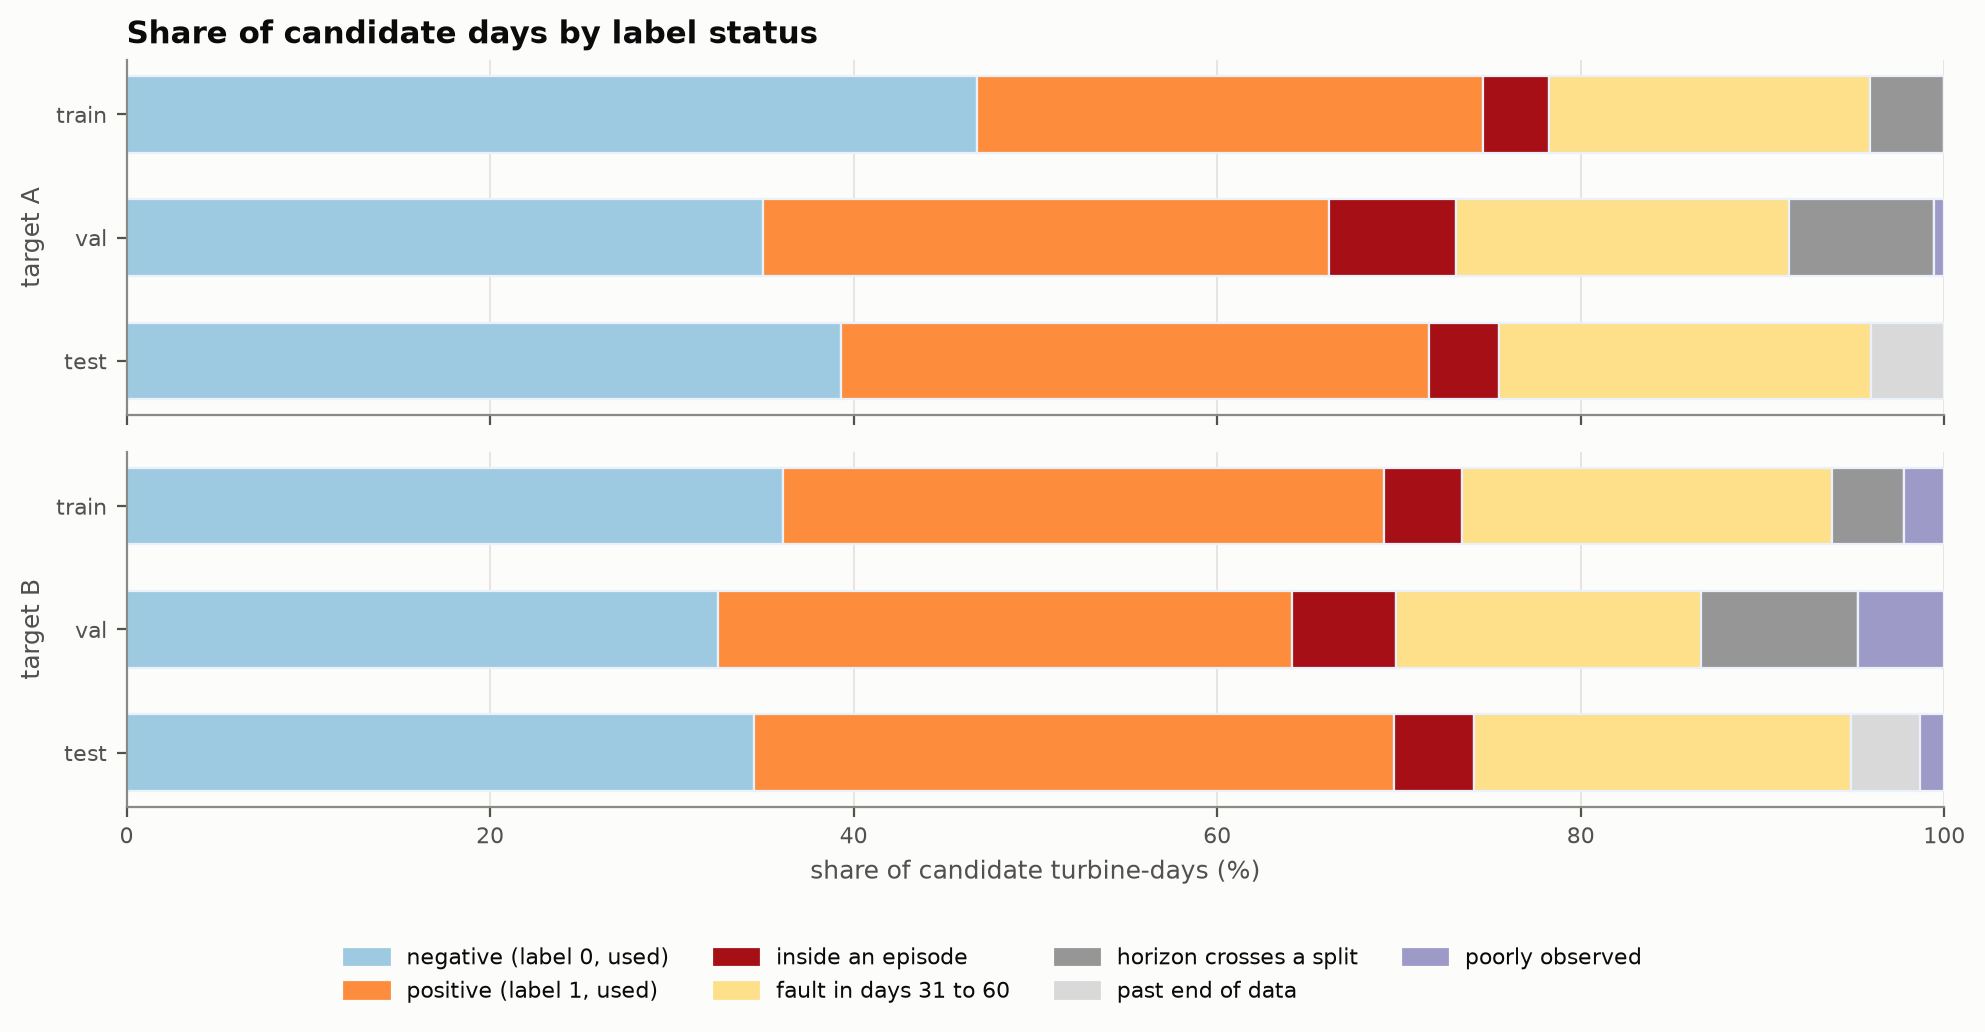
\includegraphics[width=0.85\linewidth]{02_labels/F09_label_status_by_split.png}
	\caption{Top (F08): the label windows as implemented. Bottom (F09): the share of candidate days that are labelled, and why the others are dropped.}
	\label{fig:labelstatus}
	\end{figure}

	\begin{figure}[htbp]
	\centering
	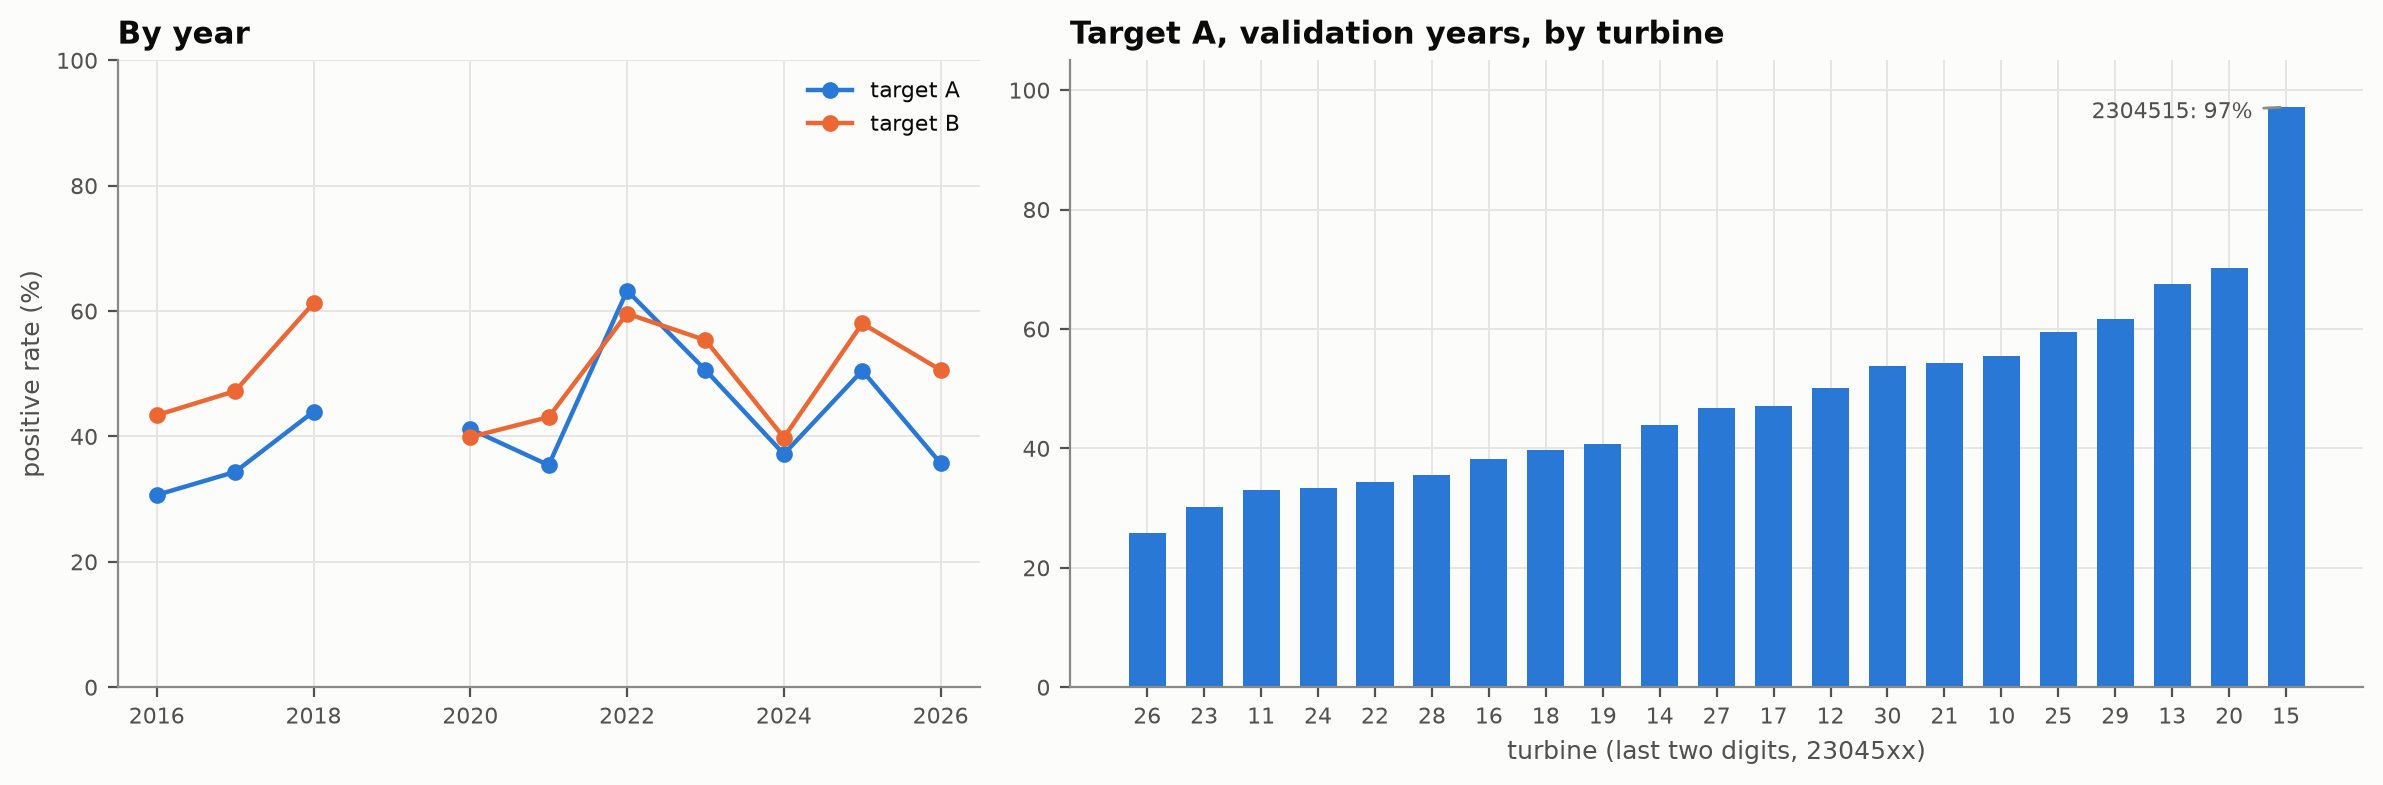
\includegraphics[width=0.9\linewidth]{02_labels/F10_positive_rate_year_turbine.png}
	\caption{Positive rate by year and by turbine (F10). The rate is 37\% to 50\% and varies by year; one turbine is positive on almost every validation day.}
	\label{fig:positive}
	\end{figure}

	\subsection{Feature Extraction}
	Each row is one turbine-day, built from data up to the end of that day. For every sensor we take the daily mean over producing intervals (generator speed at least 1000\,rpm, and at least two hours of them) and the daily maximum, plus the fractions of the day producing, idle and stopped, and wind and rotor-speed summaries. For the 7-day window we add the trailing mean and standard deviation (at least four observed days), the count of each of the 12 documented alarm codes, of each alarm tier and of all alarms in the last 7 days, and the days since and the number of fault days in the last 30 days. The table has 70{,}816 turbine-days and 366 features; each model starts from 256 candidate columns, of which about 225 remain after the training-year filter on missing and constant columns. Some sensors exist only in some years, so columns and imputation values are chosen on the training years only (Figure~\ref{fig:sensors}).

	\begin{figure}[htbp]
	\centering
	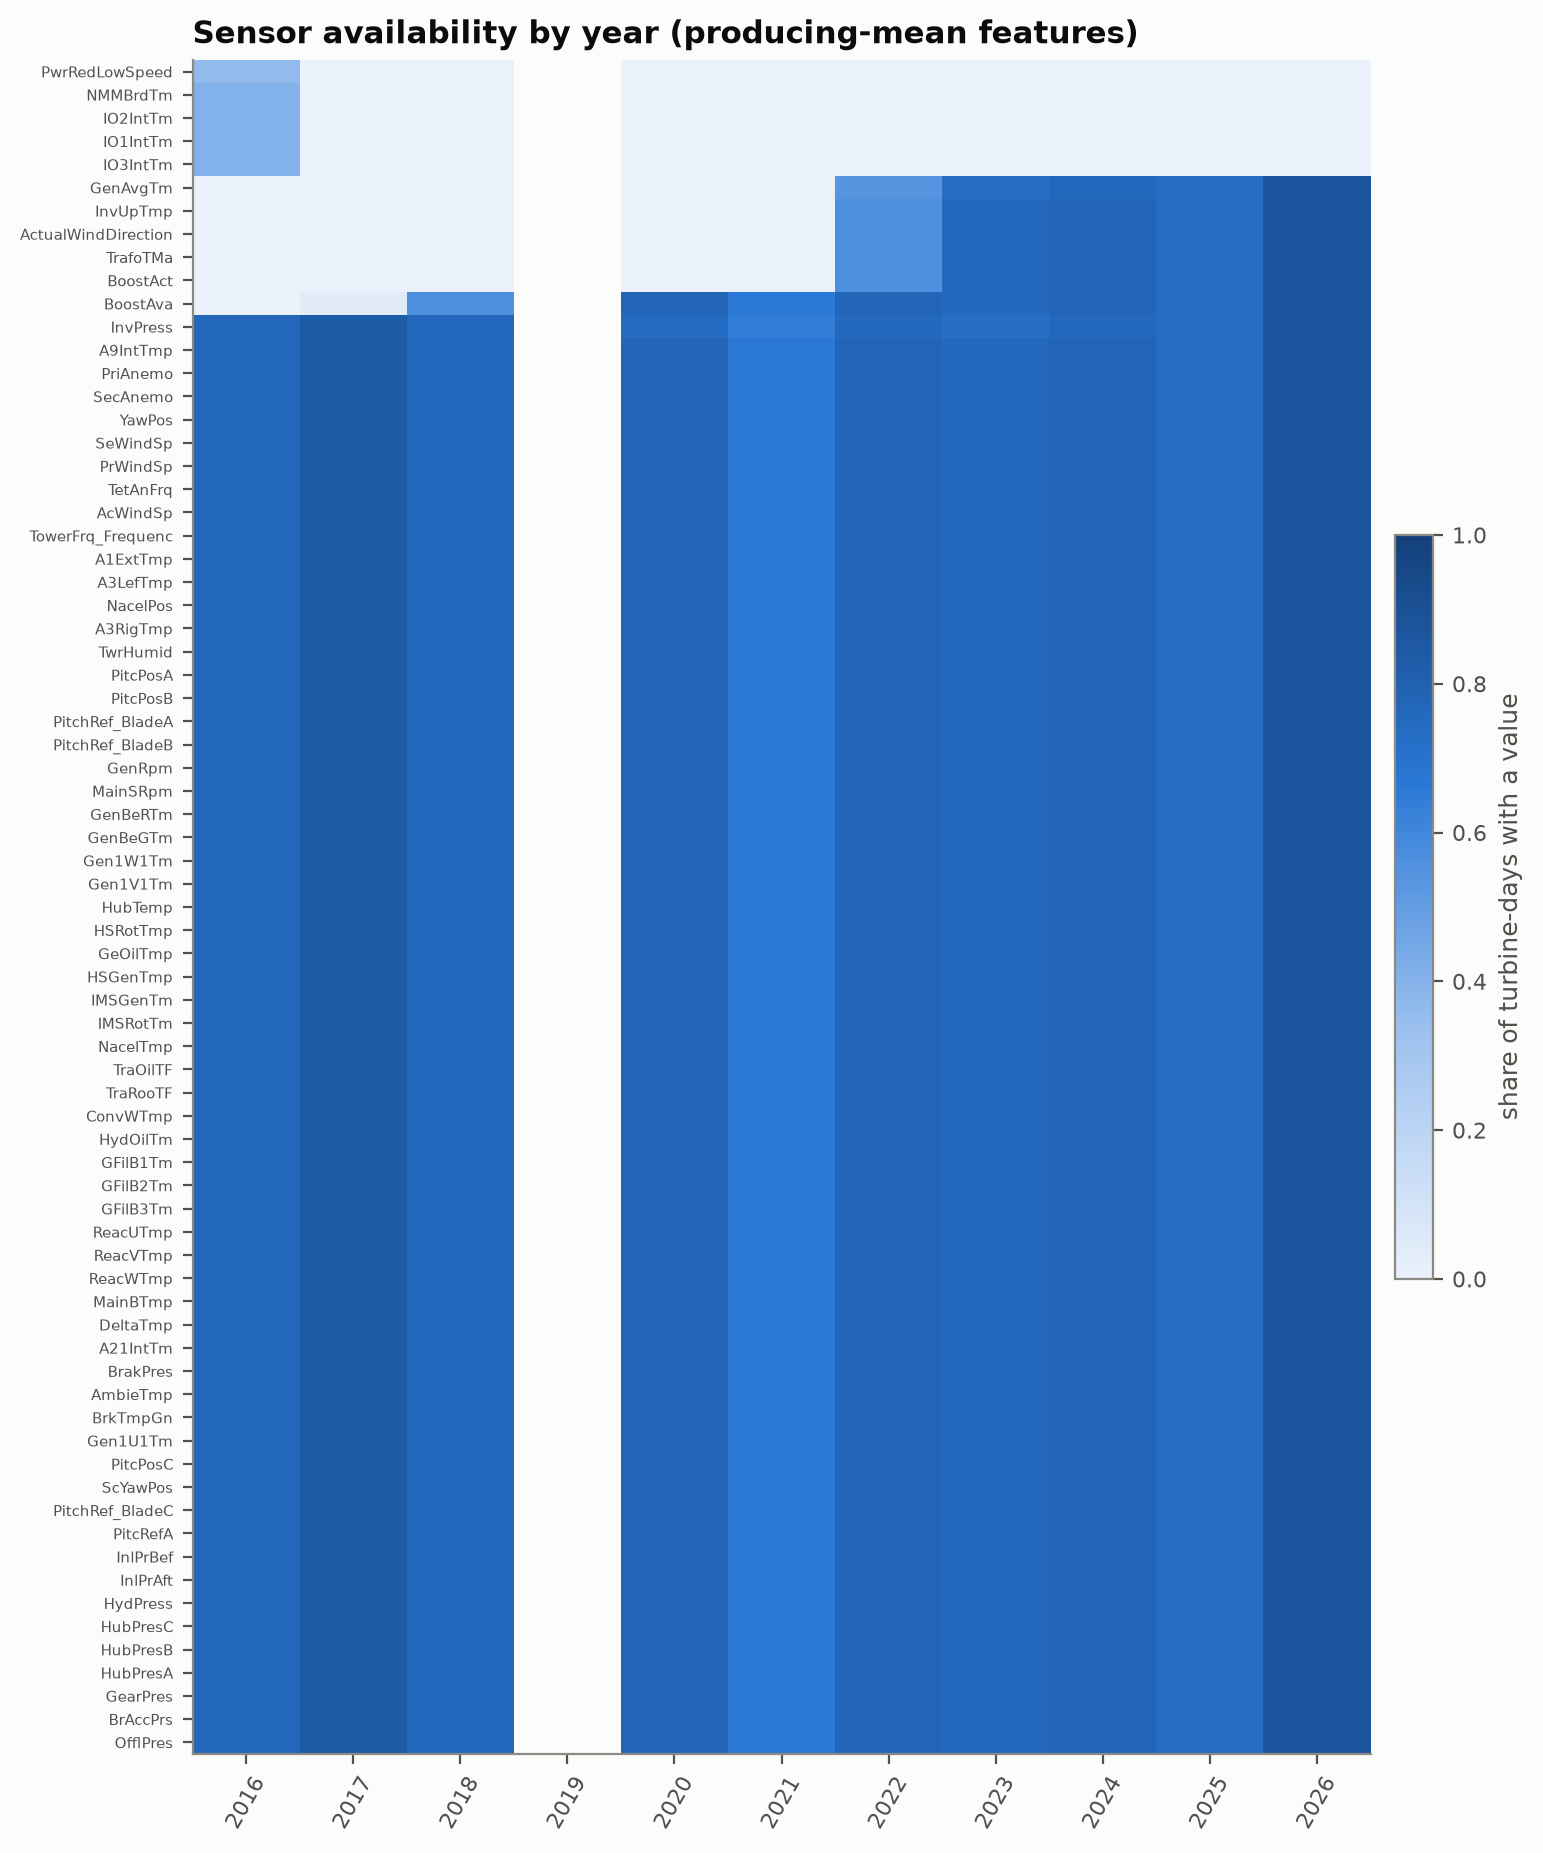
\includegraphics[width=0.85\linewidth]{03_features/F12_sensor_availability_by_year.png}
	\caption{Share of turbine-days with a value, by sensor and year (F12). Sensors appear and disappear between years.}
	\label{fig:sensors}
	\end{figure}

	\subsection{Models}\label{sec:models}
	All models score every day that has features; only labelled days enter fitting and metrics. We compare:
	\begin{itemize}
		\item \textbf{Floors:} a constant score and a random score. The random score is the reference for every result.
		\item \textbf{B1 (rule):} recent fault history, $\text{fault days in the last 30 days} + 0.5/(1+\text{days since the last fault day})$, plus its two single-column parts. It uses target A's history for both targets and is not fitted.
		\item \textbf{B2 (rule):} the 7-day alarm counts. The variant (total, tier 2, tiers 1 and 2, or one of the twelve codes) was selected per target on validation PR-AUC, so its validation value is optimistic.
		\item \textbf{B3:} a pooled healthy curve of generator speed against wind speed (0.5\,m/s bins over 4--25\,m/s, median healthy speed per bin, fitted on healthy training intervals, Figure~\ref{fig:b3}); the score is the trailing 7-day share of intervals whose shortfall exceeds twice the healthy spread. It is a proxy for under-performance, not a measured power curve.
		\item \textbf{R1:} for a set of seven bearing, oil and winding temperatures, the largest absolute z-score of the 7-day mean against the turbine's own healthy history (pooled moments for a turbine with fewer than 30 healthy days).
		\item \textbf{B4:} class-weighted logistic regression with train-only scaling and imputation; the regularisation strength ($C=0.01$) was chosen on validation.
		\item \textbf{R2 and the normal-behaviour model (O1):} ridge regressions that predict ten temperatures (gearbox oil, generator bearings, main bearing, three stator windings, transformer oil, hydraulic oil and one further drivetrain bearing) from wind speed, generator and main-shaft speed, ambient and nacelle temperature, fitted on healthy training days (7{,}635 days that are healthy for both targets, with turbine 2304515 left out of the fit but still scored; 5{,}718 had every input). The residual is predicted minus observed, divided by the turbine's healthy spread, and is made relative to the median of the turbines observed that day, which removed most of the drift between the training and validation years (mean absolute drift 0.44 to 0.06 standard deviations). The indicator is the largest absolute 7-day smoothed residual; R2 scores each day with it.
		\item \textbf{L1:} class-weighted LightGBM on the B4 columns (with and without the normal-behaviour columns), with the positive weight and the columns chosen on the training years. A grid of six settings (leaves and number of trees) was run on the validation years only and the winners were frozen (target A: 7 leaves, 300 trees; target B: 31 leaves, 300 trees).
	\end{itemize}
	Healthy days are labelled days that are not near an episode (seven days after one ends are excluded), have clean quality flags and lie in the training years.

	\begin{figure}[htbp]
	\centering
	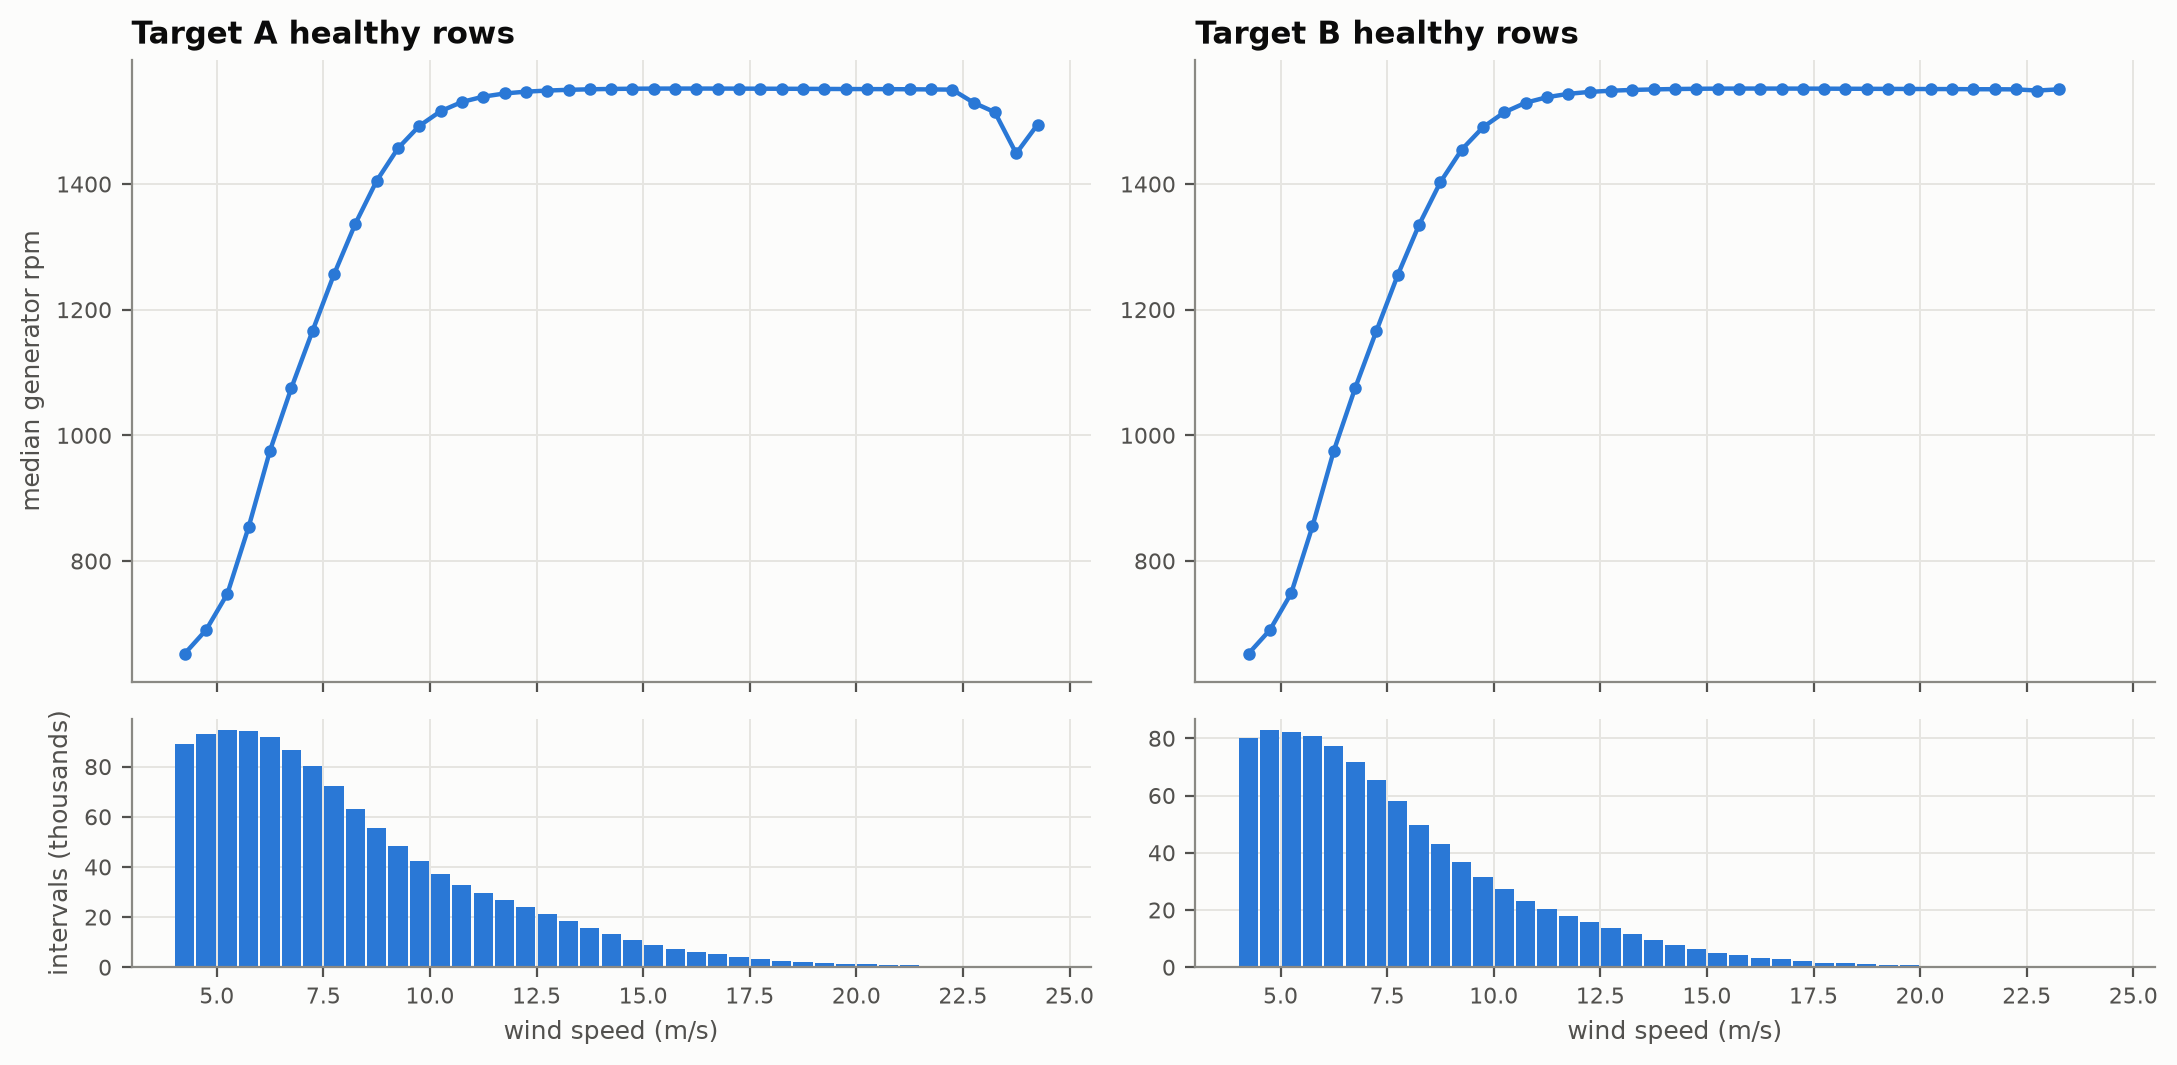
\includegraphics[width=0.85\linewidth]{05_baselines/F21_b3_power_curve.png}
	\caption{B3: the learned healthy curve of generator speed against wind speed (F21).}
	\label{fig:b3}
	\end{figure}

	\subsection{Evaluation Environment}\label{sec:evalenv}
	Models are fitted on 2016 to 2018 and 2020, settings and thresholds are chosen on 2021 to 2022, and the test years (2023 to April 2026) are scored once, for the frozen configurations (Table~\ref{tab:split}). The threshold allows at most one false-alert day per turbine-month of labelled exposure on the validation years (ties can leave budget unused) and is carried unchanged to the test years. An episode counts as detected if an alert falls 1 to 30 days before its start. Intervals come from 1{,}000 resamples of whole turbines with the threshold held fixed; they do not include the uncertainty of choosing the model or the threshold, and they treat days of one turbine as dependent but turbines as independent. The project is written in Python (pandas, scikit-learn, LightGBM, SHAP); all randomness is seeded from the configuration file. \tbc{Hardware and run times.}

	\begin{table}[htbp]
	\centering
	\small
	\begin{tabular}{@{}ll@{}}
	\toprule
	Split & Years \\
	\midrule
	Train & 2016, 2017, 2018, 2020 (2019 has no temperature or pressure tables) \\
	Validation & 2021, 2022 \\
	Test & 2023, 2024, 2025, 2026 (to April 2026) \\
	\bottomrule
	\end{tabular}
	\caption{Chronological split.}
	\label{tab:split}
	\end{table}

	\subsection{Explanation and Robustness}
	We explain the frozen LightGBM with SHAP on 4{,}000 validation days and measure how stable the ranking is by refitting without each of the 21 turbines in turn. Robustness is tested on the validation years only: refitting without one turbine and scoring that turbine (leave-one-turbine-out), and setting the features of one sensor group (pressure, drivetrain temperature, power electronics, wind and rotor speed) to missing at scoring time, at the threshold of the intact model.

	\subsection{Exploratory Follow-up Protocol}\label{sec:explmeth}
	After the frozen test run showed no model above the random score, we asked four questions, one per round, each pre-registered and each run on the validation years only (Table~\ref{tab:rounds}). The rules were the same for all rounds. Every configuration in the registered grid is run and reported; none is selected; nothing is retuned for the new setting; the models are the frozen ones (except where a round states otherwise); and the test years are never scored, so the frozen results cannot change. Each round has a year-shift check on training years only (fit on years up to 2018, score 2020) where applicable, because validation alone proved a poor guide. A turbine-ranking metric, closer to how a planner would use a score, was added in round 2: each day, among the turbines that have a label, how often are the top three by score in a positive period, compared with the share of positive turbines that day, with intervals from resampling calendar months.

	\begin{table}[htbp]
	\centering
	\footnotesize
	\begin{tabularx}{\linewidth}{@{}clXrl@{}}
	\toprule
	Round & Decision & Question and change & Configs & Best validation PR-AUC (floor) \\
	\midrule
	1 & D-064 & Do features made relative to the fleet, or very small models, cope better with drift between years? & 42 & 0.529 B (0.483) \\
	2 & D-065 & Does each turbine's own trailing 90-day median work as a baseline? Do scores rank the turbines? & 28 & 0.516 B (0.483) \\
	3 & D-066 & Which of the roughly 250 inputs matter? Do three train-only rankings, kept to 10 to 100 columns, help? & 132 & 0.530 B (0.483) \\
	4 & D-068 & Are the labels the bottleneck? 27 label definitions, each against its own floor. & 189 & see Section~\ref{sec:labelsens} \\
	\bottomrule
	\end{tabularx}
	\caption{The four exploratory rounds. Configurations are model-by-setting runs on the validation years (round 3 includes 96 pruned runs, 28 group-removal runs and 8 all-column references; round 4 is 27 variants of seven models).}
	\label{tab:rounds}
	\end{table}

	%===========================================================
	\section{Simulation Results}\label{sec:findings}
	\subsection{Key Findings and Significance}

	\paragraph{Validation years.} On the tuning years the per-turbine z-score R1 had the highest PR-AUC for both targets (0.577 for A and 0.588 for B, against random scores of 0.465 and 0.483), and recall-based comparisons with the random score were below it for every model (Table~\ref{tab:valtest}). The supervised models, B4 and LightGBM, were below the random-score value on validation.

	\paragraph{Test years.} Tables~\ref{tab:testa} and~\ref{tab:testb} give the single scored run on the test years. The random-score PR-AUC is 0.450 for target A and 0.506 for target B, and \textbf{the 95\% interval of every model contains it}. The highest point estimates are for LightGBM (0.492 and 0.493 with the normal-behaviour columns for A; 0.556 for B) and for logistic regression on target B (0.563). These are about 0.04 above the best simple rule (B2 at 0.453 for A, B3 at 0.517 for B), but the intervals overlap both the rules and the random-score value, so the learned models are ahead only in the point estimates. R1 falls from 0.577 and 0.588 on validation to 0.448 and 0.499 on test, so its advantage did not hold (Figure~\ref{fig:valtest}). No model reaches the random-score episode recall (0.795 and 0.839) at a comparable false-alarm rate; the models that reach recall of 0.55 to 0.68 (R1 and R2) do so at 2.1 to 2.5 false alarms per turbine-month, about twice the budget, because the validation threshold does not carry over. The median lead times of 17 to 30 days are close to the 21 days of a random score.

	\begin{figure}[htbp]
	\centering
	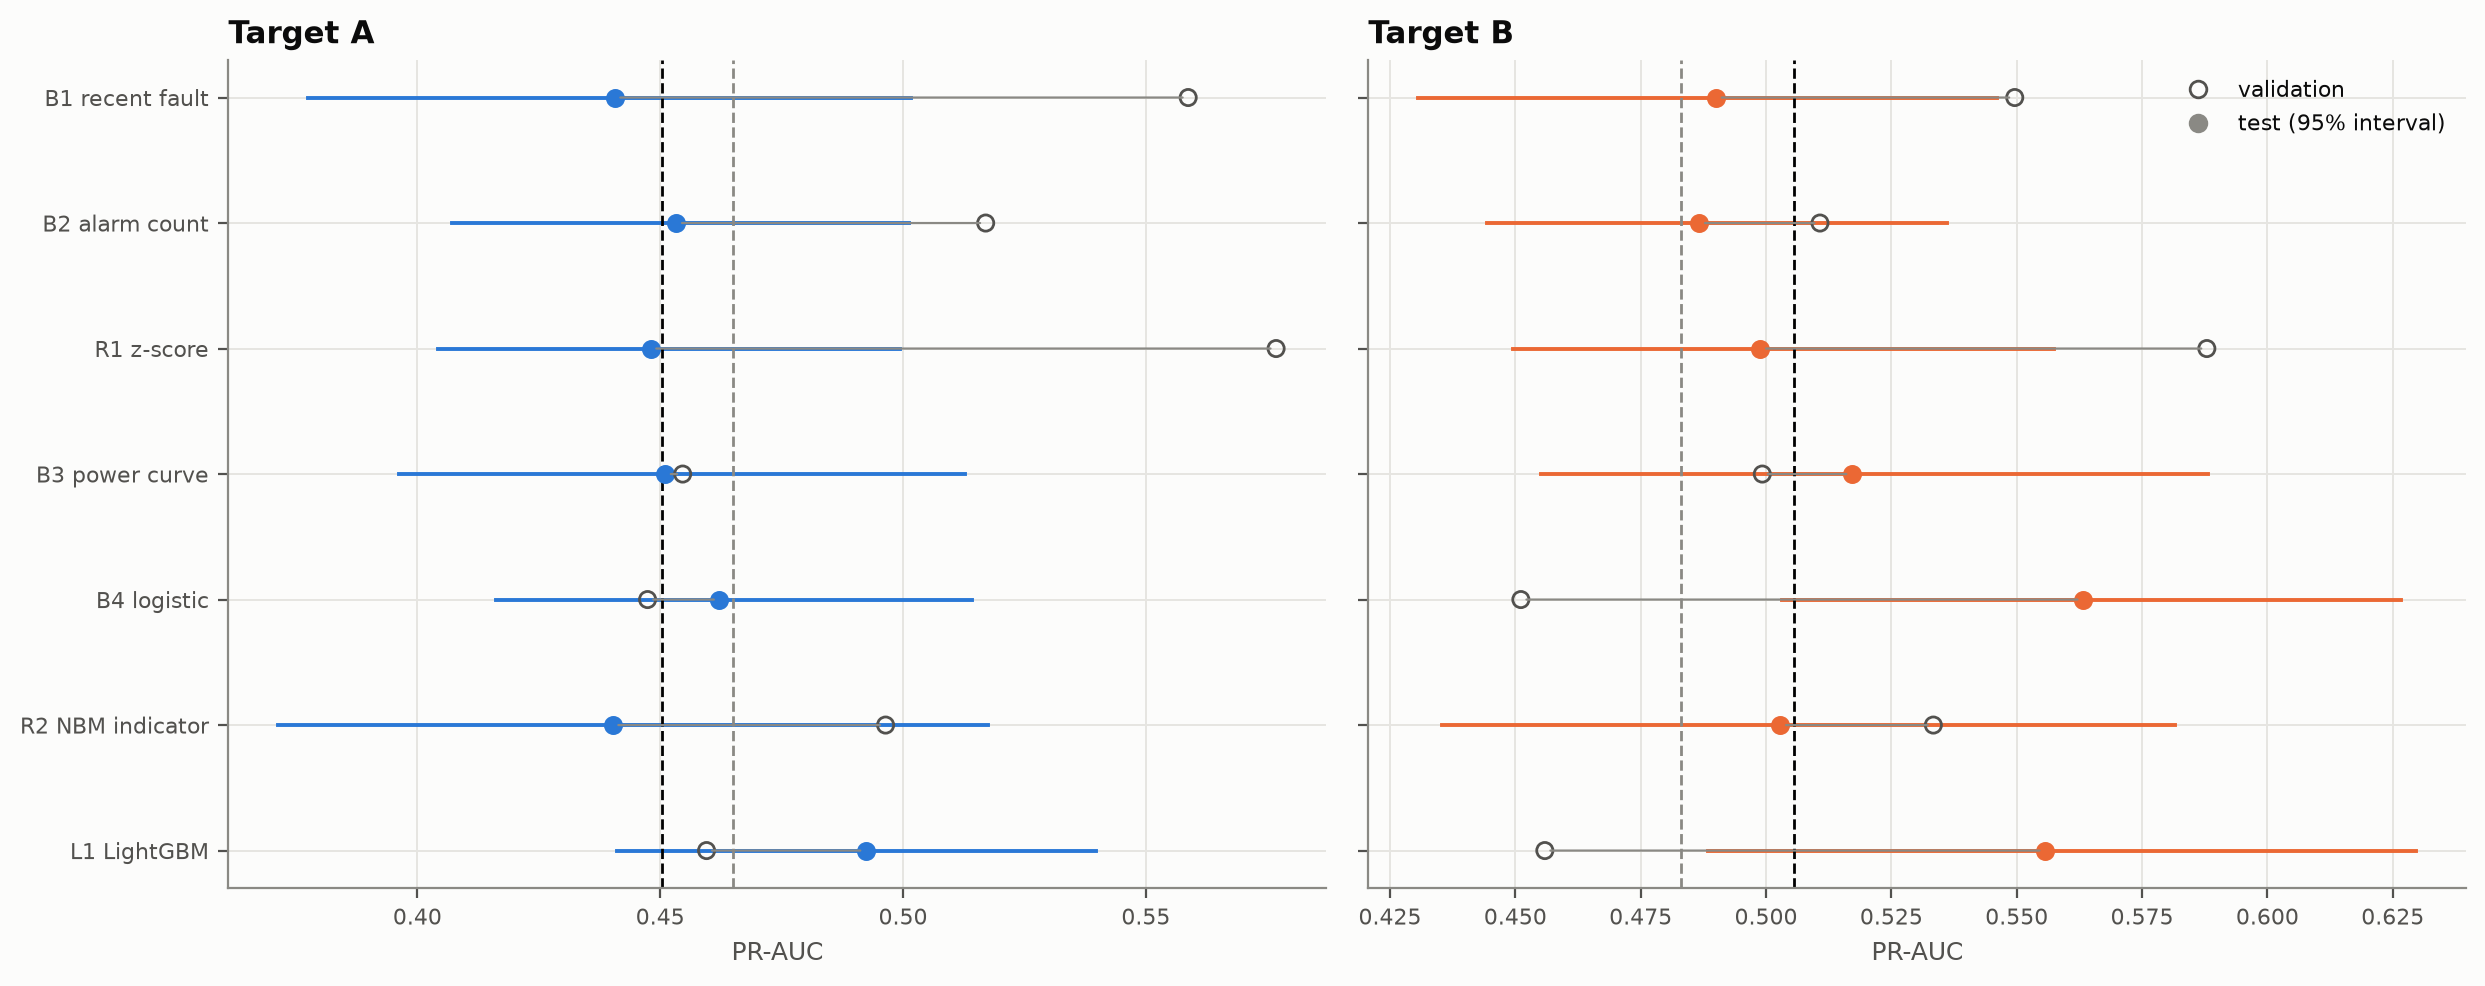
\includegraphics[width=\linewidth]{08_exploratory/F36_validation_to_test_shift.png}
	\caption{From validation to test (F36). Hollow: validation PR-AUC; filled with line: test PR-AUC with its 95\% interval. Dashed lines are the random-score values (grey: validation; black: test). The ranking on validation did not carry over to test.}
	\label{fig:valtest}
	\end{figure}

	\begin{table}[htbp]
	\centering
	\small
	\begin{tabular}{@{}lcccc@{}}
\toprule
 & \multicolumn{2}{c}{Target A} & \multicolumn{2}{c}{Target B} \\
\cmidrule(lr){2-3}\cmidrule(lr){4-5}
Model & Validation & Test & Validation & Test \\
\midrule
Random score & 0.465 & 0.450 & 0.483 & 0.506 \\
B1 recent fault & 0.559 & 0.441 & 0.550 & 0.490 \\
B1 fault count & 0.533 & 0.451 & 0.530 & 0.501 \\
B1 fault recency & 0.528 & 0.444 & 0.531 & 0.493 \\
B2 alarm count & 0.517 & 0.453 & 0.511 & 0.487 \\
R1 z-score & 0.577 & 0.448 & 0.588 & 0.499 \\
B3 power curve & 0.455 & 0.451 & 0.499 & 0.517 \\
B4 logistic & 0.447 & 0.462 & 0.451 & 0.563 \\
R2 NBM indicator & 0.496 & 0.440 & 0.533 & 0.503 \\
L1 LightGBM & 0.460 & 0.492 & 0.456 & 0.556 \\
L1 LightGBM + NBM & 0.445 & 0.493 & 0.454 & 0.547 \\
\bottomrule
\end{tabular}

	\caption{PR-AUC on the validation and test years for the full fleet. The random-score PR-AUC is 0.465 (A) and 0.483 (B) on validation, and 0.450 (A) and 0.506 (B) on test.}
	\label{tab:valtest}
	\end{table}

	\begin{table}[htbp]
	\centering
	\footnotesize
	\begin{tabular}{@{}lccc@{}}
\toprule
Model & PR-AUC [95\% interval] & Episode recall [95\% interval] & False alarms per turbine-month \\
\midrule
Random score & 0.450 [0.402, 0.504] & 0.795 [0.752, 0.839] & 0.91 \\
B1 recent fault & 0.441 [0.377, 0.502] & 0.131 [0.091, 0.170] & 0.78 \\
B1 fault count & 0.451 [0.396, 0.506] & 0.065 [0.035, 0.097] & 0.47 \\
B1 fault recency & 0.444 [0.388, 0.497] & 0.360 [0.314, 0.402] & 0.95 \\
B2 alarm count & 0.453 [0.407, 0.501] & 0.271 [0.220, 0.323] & 0.62 \\
R1 z-score & 0.448 [0.404, 0.499] & 0.622 [0.564, 0.680] & 2.12 \\
B3 power curve & 0.451 [0.396, 0.513] & 0.235 [0.178, 0.292] & 0.68 \\
B4 logistic & 0.462 [0.416, 0.514] & 0.202 [0.121, 0.286] & 0.43 \\
R2 NBM indicator & 0.440 [0.371, 0.517] & 0.551 [0.472, 0.635] & 2.53 \\
L1 LightGBM & 0.492 [0.441, 0.540] & 0.211 [0.143, 0.288] & 0.28 \\
L1 LightGBM + NBM & 0.493 [0.445, 0.540] & 0.217 [0.148, 0.296] & 0.25 \\
\bottomrule
\end{tabular}

	\caption{Test years, target A: 17{,}947 scored days (of 17{,}951 labelled), 8{,}097 positive, 336 episodes. Random-score values: PR-AUC 0.450, episode recall 0.795. The 95\% intervals resample turbines (\texttt{reports/TEST\_RESULTS.md}).}
	\label{tab:testa}
	\end{table}

	\begin{table}[htbp]
	\centering
	\footnotesize
	\begin{tabular}{@{}lccc@{}}
\toprule
Model & PR-AUC [95\% interval] & Episode recall [95\% interval] & False alarms per turbine-month \\
\midrule
Random score & 0.506 [0.457, 0.564] & 0.839 [0.804, 0.873] & 0.85 \\
B1 recent fault & 0.490 [0.431, 0.546] & 0.155 [0.123, 0.190] & 0.74 \\
B1 fault count & 0.501 [0.450, 0.553] & 0.139 [0.106, 0.172] & 0.72 \\
B1 fault recency & 0.493 [0.437, 0.547] & 0.362 [0.312, 0.411] & 1.09 \\
B2 alarm count & 0.487 [0.444, 0.536] & 0.174 [0.142, 0.208] & 0.48 \\
R1 z-score & 0.499 [0.449, 0.557] & 0.676 [0.617, 0.732] & 2.15 \\
B3 power curve & 0.517 [0.455, 0.588] & 0.279 [0.217, 0.340] & 0.77 \\
B4 logistic & 0.563 [0.503, 0.627] & 0.220 [0.155, 0.294] & 0.34 \\
R2 NBM indicator & 0.503 [0.435, 0.582] & 0.635 [0.568, 0.695] & 2.42 \\
L1 LightGBM & 0.556 [0.488, 0.630] & 0.354 [0.264, 0.448] & 0.66 \\
L1 LightGBM + NBM & 0.547 [0.477, 0.622] & 0.354 [0.270, 0.439] & 0.72 \\
\bottomrule
\end{tabular}

	\caption{Test years, target B: 17{,}281 labelled days, 8{,}725 positive, 373 episodes evaluated (382 in Table~\ref{tab:labels}; \tbc{confirm why nine episodes are not evaluated}). Random-score values: PR-AUC 0.506, episode recall 0.839.}
	\label{tab:testb}
	\end{table}

	\begin{figure}[htbp]
	\centering
	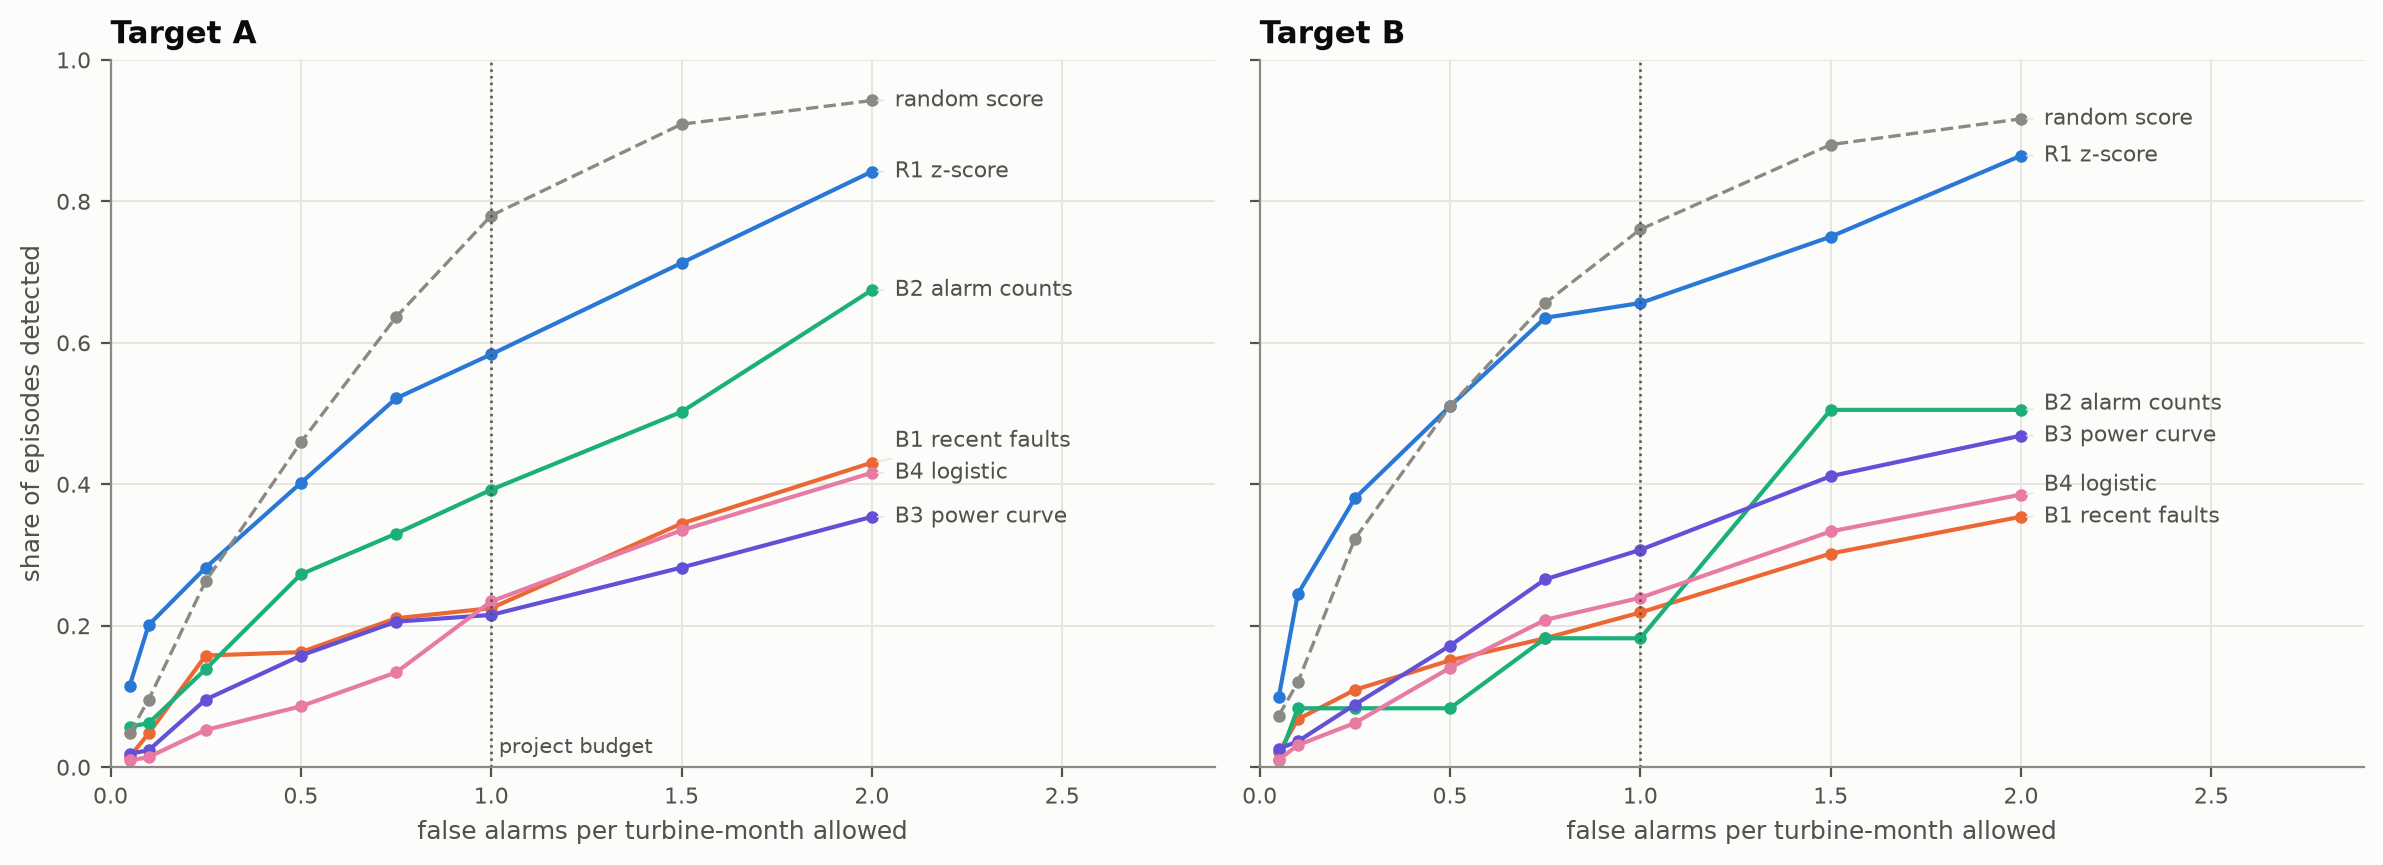
\includegraphics[width=0.95\linewidth]{04_evaluation/F15_recall_vs_false_alarm_budget.png}
	\caption{Episode recall against the false-alarm budget on the validation years (F15). Only R1 is above the random line, and only at the tightest budgets.}
	\end{figure}

	\paragraph{O1: degradation indicator.} The normal-behaviour models fit the healthy training days well for the stator windings (R-squared 0.95) and poorly for the hydraulic oil (0.11). Before the fleet-relative correction, the standardised residuals on healthy-looking validation days had a mean of up to 0.9 standard deviations away from zero, so part of any signal is drift between years (Figure~\ref{fig:nbm}, top). After it the drift is within about 0.2. The indicator is only slightly higher in the 30 days before an episode than far from one, it does not rise steadily as an episode nears, and the sensor with the largest residual is spread over several sensors in much the same way on positive and negative days (Figure~\ref{fig:nbm}, bottom). As a risk score R2 had a PR-AUC of 0.496 (A) and 0.533 (B) on validation and 0.440 and 0.503 on test, close to the random-score value.

	\begin{figure}[htbp]
	\centering
	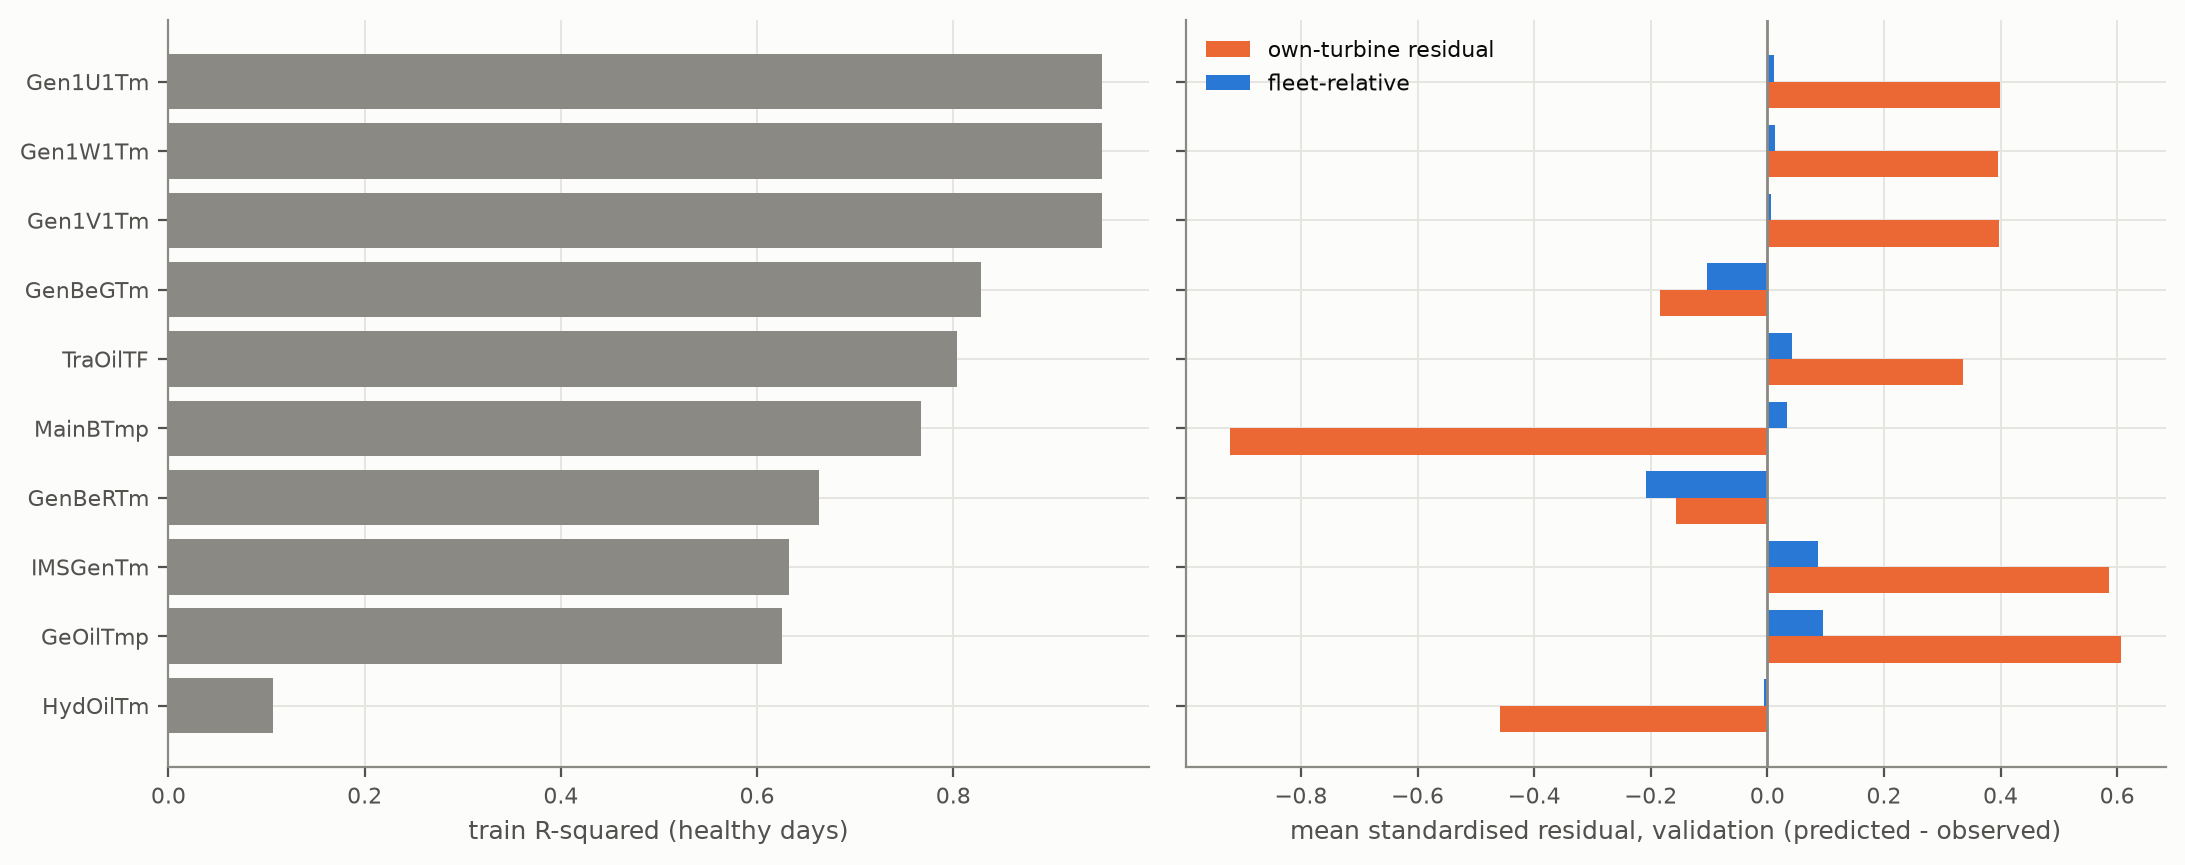
\includegraphics[width=0.95\linewidth]{06_nbm/F32_nbm_validation_shift.png}\\[4pt]
	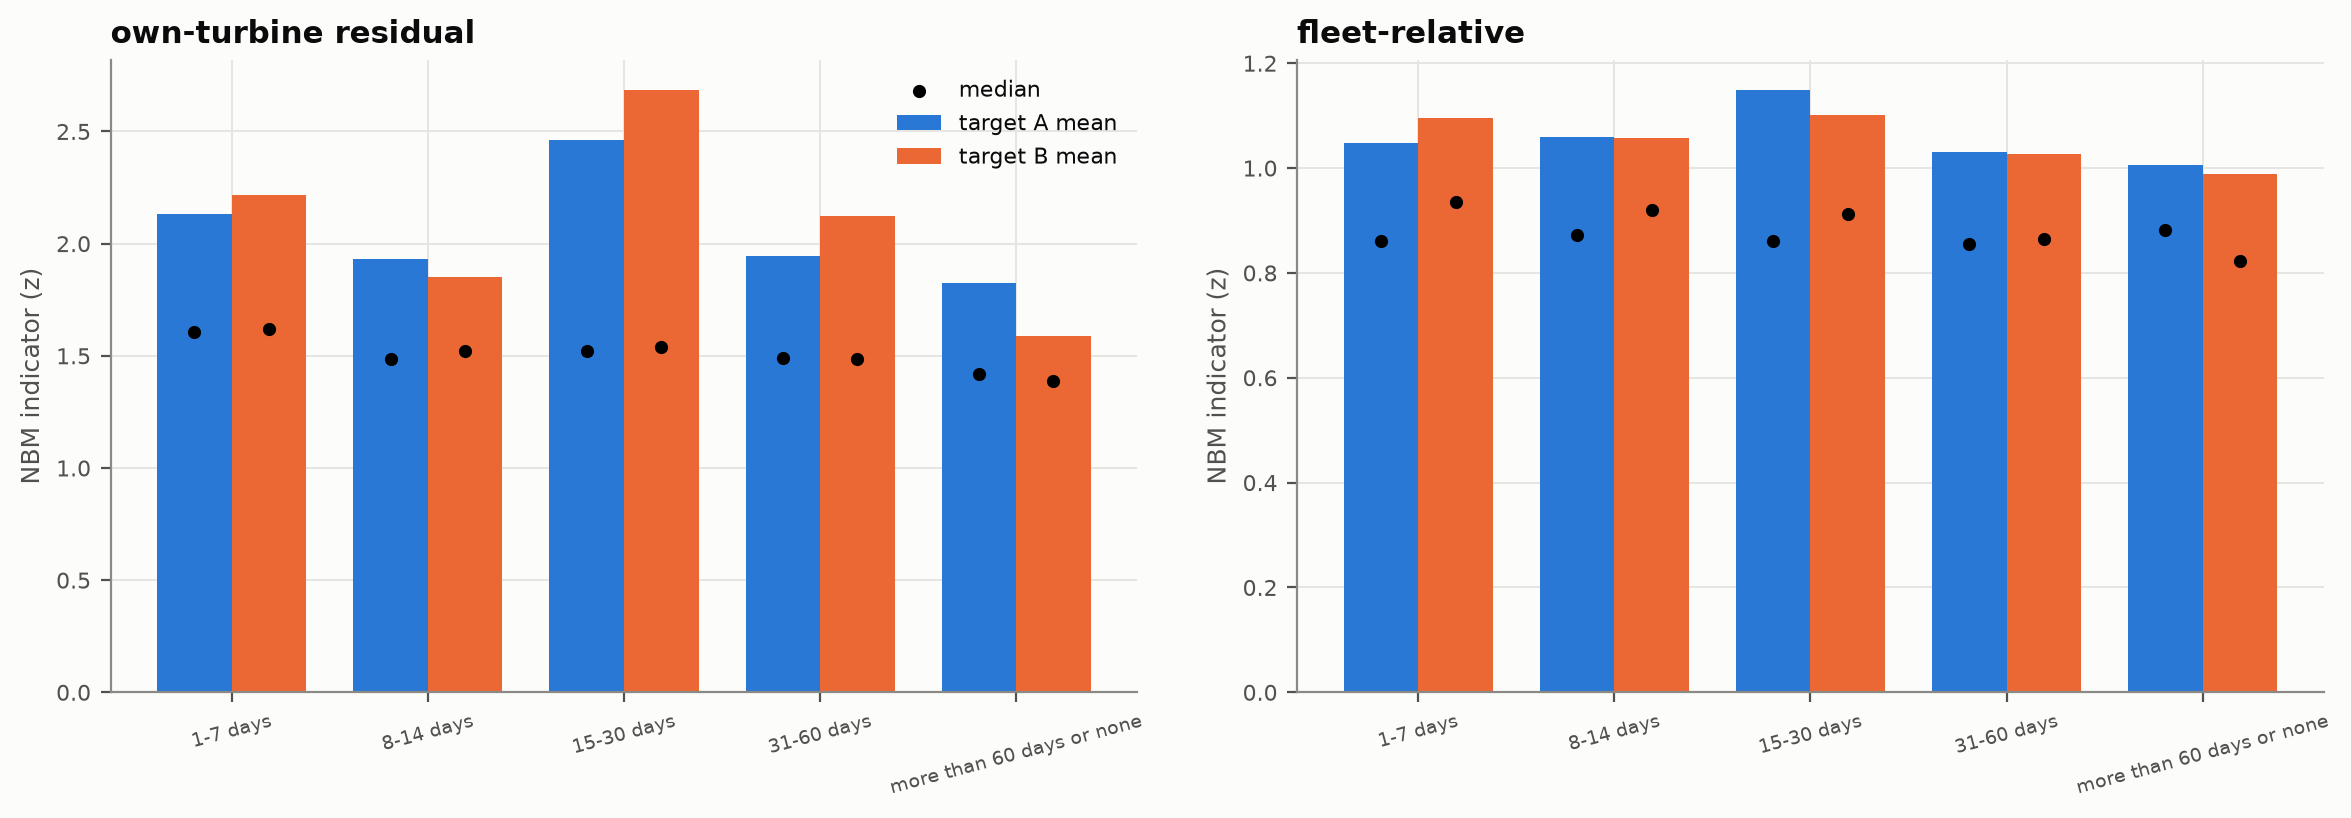
\includegraphics[width=0.95\linewidth]{06_nbm/F33_nbm_indicator_vs_lead.png}
	\caption{Normal-behaviour model on the validation years. Top (F32): training fit and validation drift per sensor. Bottom (F33): indicator against time to the next episode.}
	\label{fig:nbm}
	\end{figure}

	\paragraph{O3: robustness.} Removing any sensor group at scoring time changed the validation PR-AUC of LightGBM by at most 0.023 (Table~\ref{tab:dropout}). Recall at the fixed threshold changed more, but together with the false-alarm rate (for target B, removing the pressure group raised recall from 0.22 to 0.46 while false alarms rose from 1.0 to 2.9 per turbine-month), which is a shift in the scores and not a gain in skill. Refitting without one turbine at a time gave a pooled PR-AUC at or below the pooled prevalence (Table~\ref{tab:loto}), and the PR-AUC of single turbines followed their own prevalence (Figure~\ref{fig:robust}, bottom); every turbine has at least 113 positive validation days. We did not run the upgrade analysis, because the installation dates were not in our files. The year-shift check on training years is part of the exploratory rounds below.

	\begin{table}[htbp]
	\centering
	\small
	\begin{tabular}{@{}llcccc@{}}
\toprule
Target & Sensor group removed & PR-AUC & Change & Recall & False alarms \\
\midrule
A & None (intact model) & 0.460 &  & 0.163 & 1.00 \\
A & Pressure & 0.483 & +0.023 & 0.182 & 0.98 \\
A & Drivetrain temperature & 0.469 & +0.009 & 0.273 & 1.41 \\
A & Power electronics & 0.456 & -0.004 & 0.120 & 0.91 \\
A & Wind and rpm & 0.457 & -0.003 & 0.153 & 0.90 \\
B & None (intact model) & 0.456 &  & 0.219 & 1.00 \\
B & Pressure & 0.448 & -0.007 & 0.458 & 2.86 \\
B & Drivetrain temperature & 0.463 & +0.007 & 0.349 & 1.79 \\
B & Power electronics & 0.456 & +0.001 & 0.271 & 1.18 \\
B & Wind and rpm & 0.457 & +0.002 & 0.198 & 1.00 \\
\bottomrule
\end{tabular}

	\caption{Sensor-group dropout on the validation years at the intact model's threshold (frozen LightGBM). Change is in PR-AUC.}
	\label{tab:dropout}
	\end{table}

	\begin{table}[htbp]
	\centering
	\small
	\begin{tabular}{@{}lcccc@{}}
\toprule
Target & Left out & Full fit & Prevalence & Fewest positive days \\
\midrule
A & 0.467 & 0.460 & 0.470 & 132 \\
B & 0.447 & 0.456 & 0.492 & 113 \\
\bottomrule
\end{tabular}

	\caption{Leave-one-turbine-out on the validation years: pooled PR-AUC with each turbine left out of training, with the full fit, and the pooled prevalence.}
	\label{tab:loto}
	\end{table}

	\paragraph{O4: explanation.} The inputs LightGBM relies on most are ambient and weather-linked (\texttt{DeltaTmp}, ambient temperature, tower humidity and frequency), pressure sensors (inverter, offline and hub pressure) and the days since the last fault day; component temperatures such as the main bearing and the hydraulic oil rank lower (Figure~\ref{fig:robust}, top). The ranking is stable when a turbine is left out (median rank correlation 0.86 for A and 0.93 for B, and a median of 18 of the top 20 features shared). This describes how the model uses its inputs, not what causes faults, and because the model scores at the random level a stable ranking is not evidence of a useful signal.

	\begin{figure}[htbp]
	\centering
	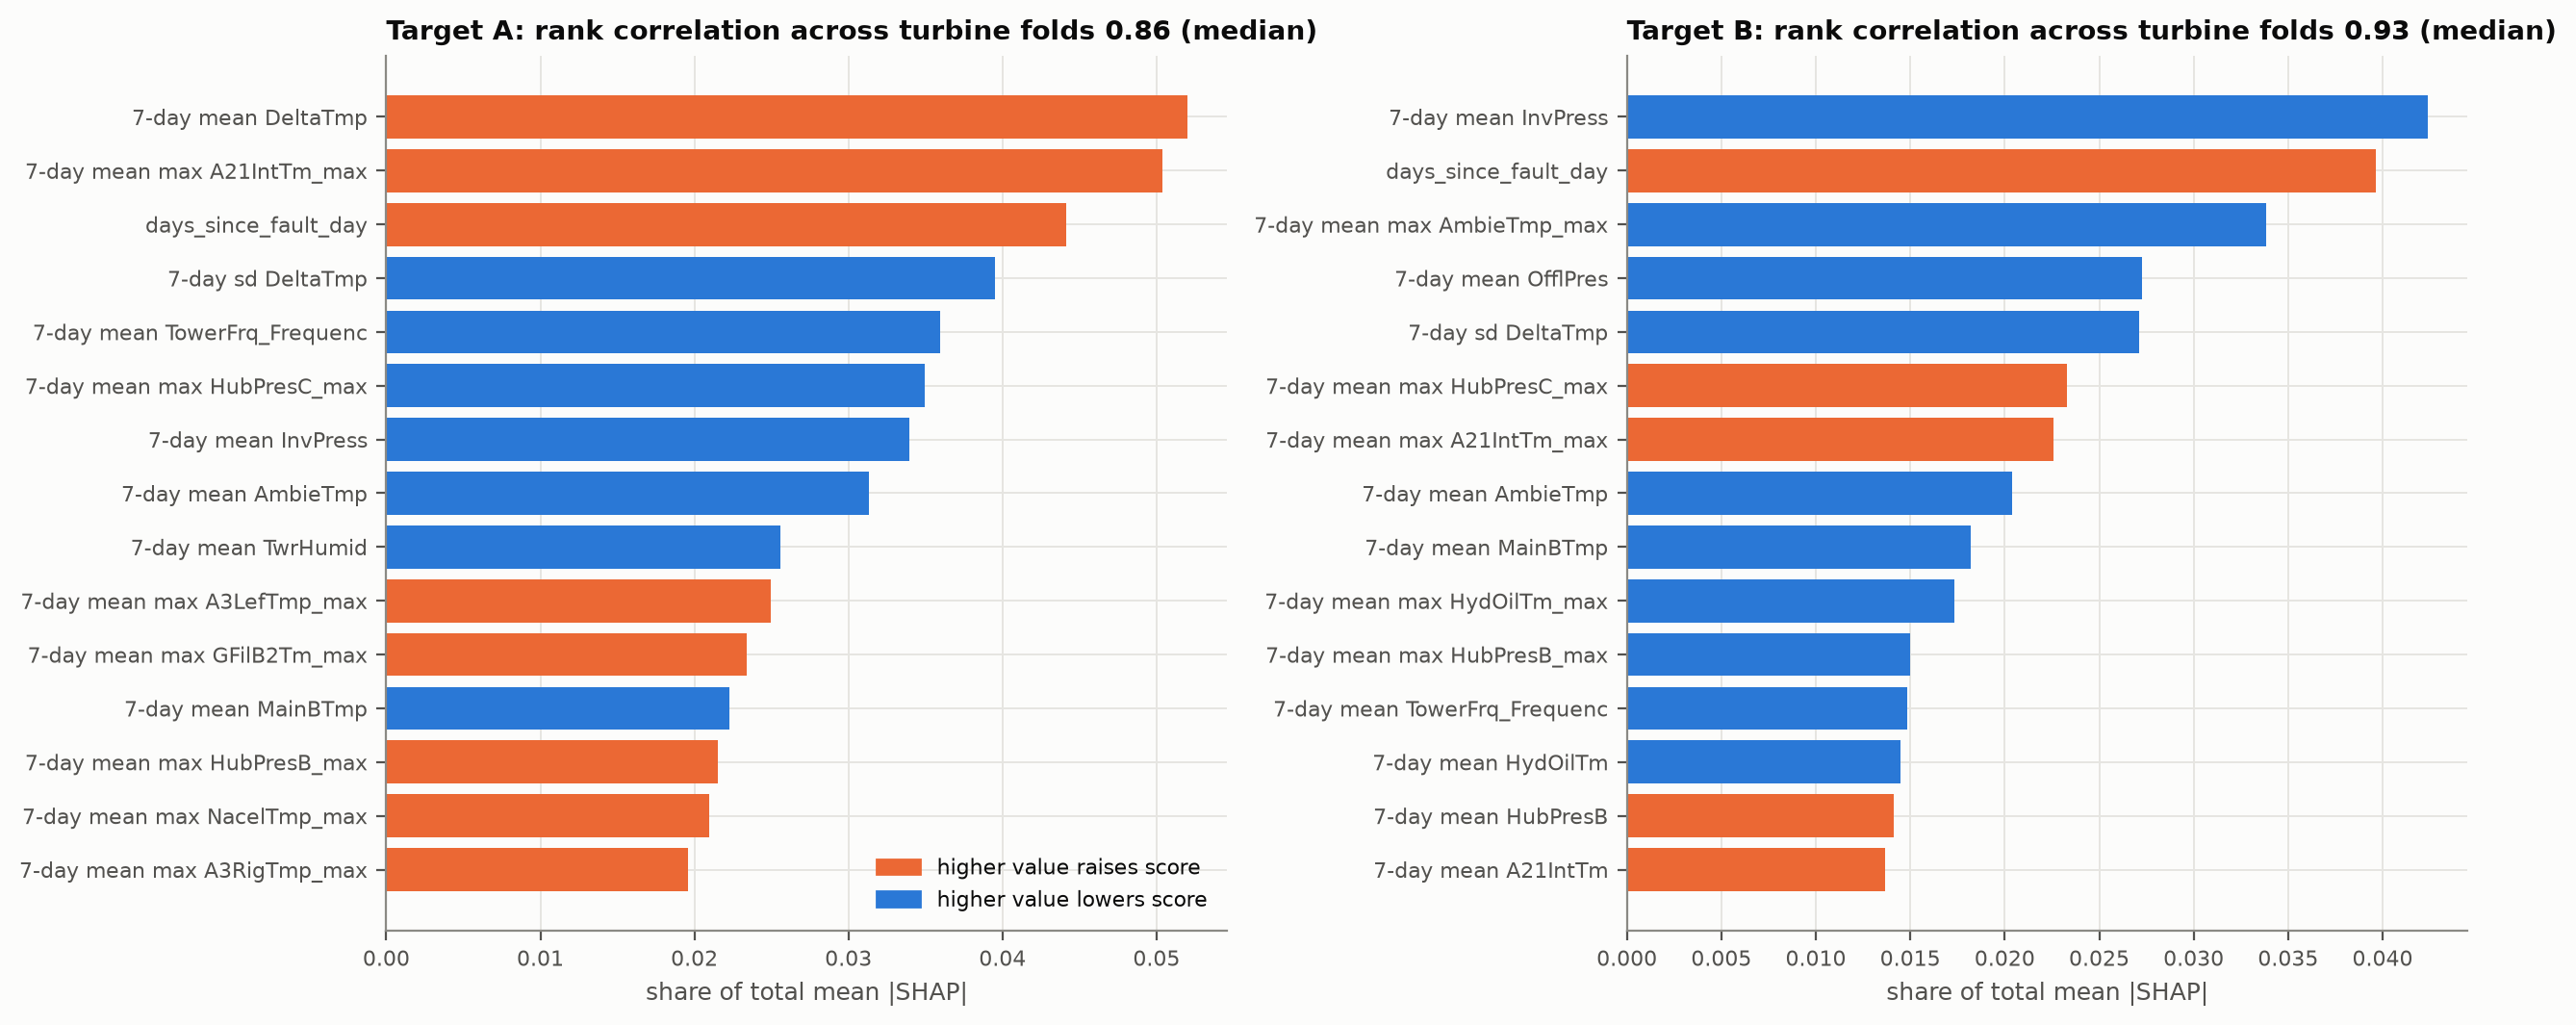
\includegraphics[width=0.95\linewidth]{07_explain_robustness/F34_shap_top_features.png}\\[4pt]
	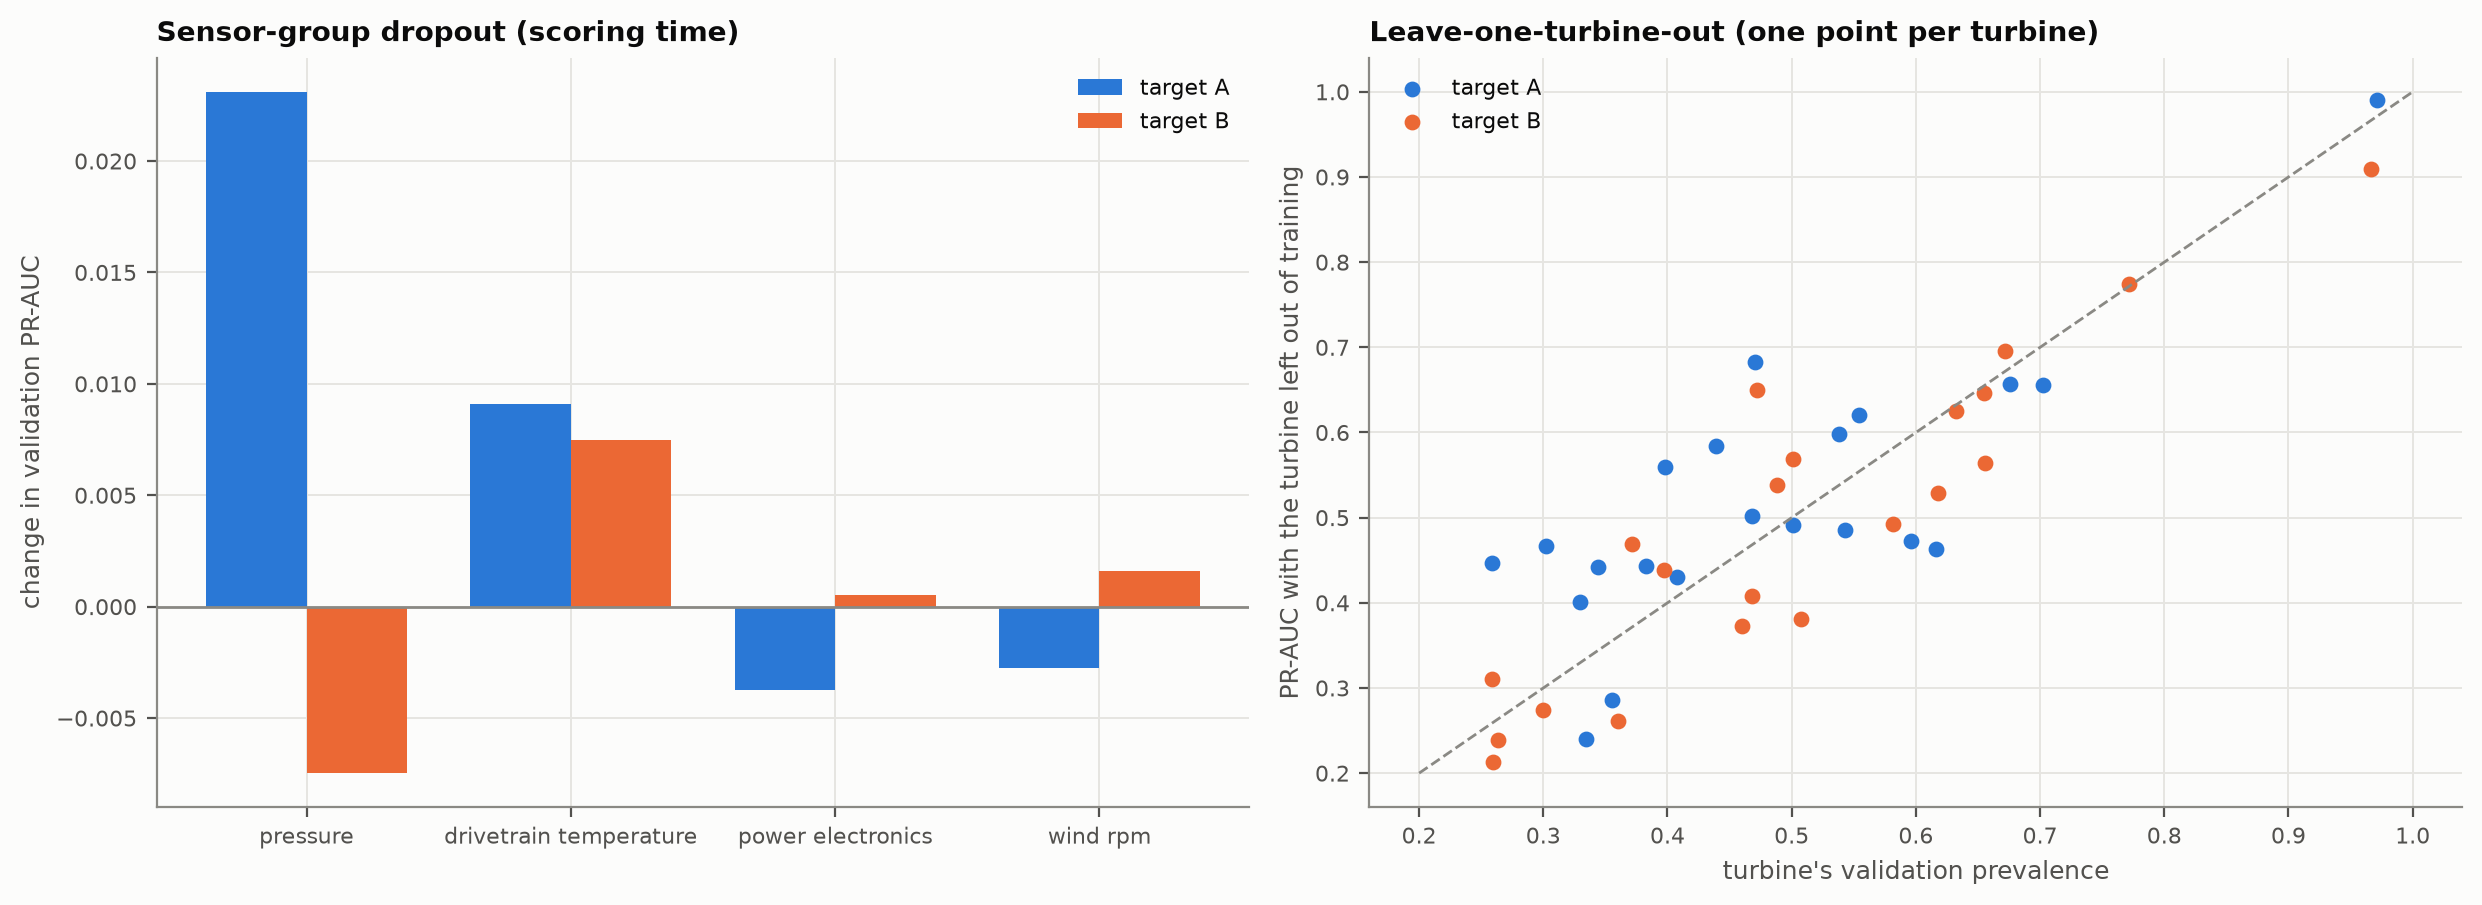
\includegraphics[width=0.95\linewidth]{07_explain_robustness/F35_robustness_dropout_loto.png}
	\caption{Validation years, frozen LightGBM. Top (F34): SHAP importance. Bottom (F35): sensor-group dropout and leave-one-turbine-out.}
	\label{fig:robust}
	\end{figure}

	\subsection{Exploratory Follow-up (validation years only)}\label{sec:explres}
	The rounds of Table~\ref{tab:rounds} were run to find out why the frozen models failed and whether any cheap change would fix it. All results below are on the validation years, where a random score has a PR-AUC of 0.465 (A) and 0.483 (B); none was scored on the test years, and with 391 model-by-setting runs in total the best are optimistically biased.

	\paragraph{Round 1: features relative to the fleet.} Each sensor-derived feature has the median of the same feature over the turbines observed that day subtracted (so no later day is used), optionally also with the training-year month-of-year mean removed; low-capacity models (LightGBM with three leaves and depth two, and L1-penalised logistic regression) were added. All 42 combinations were run and none was selected (Table~\ref{tab:explval}). Fleet-relative features raised the validation PR-AUC of the logistic models for both targets (for target A, logistic regression 0.447 to 0.483) and of the tree models for target B (LightGBM 0.456 to 0.516, very small trees 0.433 to 0.529), but not of LightGBM for target A (0.460 to 0.452); removing the month-of-year mean as well lowered the scores again in almost every case. Every 95\% interval still contains the random-score value (the highest, 0.529 for target B, has the interval [0.440, 0.618]), and recall at the budget stayed between 0.10 and 0.32 against 0.76 to 0.78 for a random score. The year-shift check (Table~\ref{tab:explshift}) puts every model with the raw features above the prevalence of 2020 (0.412 for A, 0.399 for B), and the fleet-relative features give no consistent gain there.

	\begin{table}[htbp]
	\centering
	\footnotesize
	\begin{tabular}{@{}lcccccc@{}}
\toprule
 & \multicolumn{3}{c}{Target A} & \multicolumn{3}{c}{Target B} \\
\cmidrule(lr){2-4}\cmidrule(lr){5-7}
Model (setting) & Raw & Fleet & Fleet+season & Raw & Fleet & Fleet+season \\
\midrule
L1 LightGBM (frozen) (D-060) & 0.460 & 0.452 & 0.414 & 0.456 & 0.516 & 0.441 \\
B4 logistic (frozen) (D-041) & 0.447 & 0.483 & 0.466 & 0.451 & 0.516 & 0.496 \\
Shallow trees (50 trees, depth 2) & 0.408 & 0.446 & 0.402 & 0.433 & 0.529 & 0.422 \\
Shallow trees (150 trees, depth 2) & 0.419 & 0.441 & 0.402 & 0.435 & 0.518 & 0.420 \\
Sparse logistic (L1) (C=0.003) & 0.428 & 0.482 & 0.467 & 0.452 & 0.507 & 0.495 \\
Sparse logistic (L1) (C=0.01) & 0.455 & 0.478 & 0.463 & 0.451 & 0.515 & 0.490 \\
Sparse logistic (L1) (C=0.03) & 0.453 & 0.481 & 0.460 & 0.454 & 0.519 & 0.493 \\
\bottomrule
\end{tabular}

	\caption{Round 1, validation PR-AUC. Raw: features as in the main models; Fleet: sensor features minus the same-day fleet median; Fleet+season: also minus the training-year month-of-year mean. Random-score value: 0.465 (A) and 0.483 (B).}
	\label{tab:explval}
	\end{table}

	\begin{table}[htbp]
	\centering
	\footnotesize
	\begin{tabular}{@{}lcccccc@{}}
\toprule
 & \multicolumn{3}{c}{Target A} & \multicolumn{3}{c}{Target B} \\
\cmidrule(lr){2-4}\cmidrule(lr){5-7}
Model (setting) & Raw & Fleet & Fleet+season & Raw & Fleet & Fleet+season \\
\midrule
L1 LightGBM (frozen) (D-060) & 0.466 & 0.432 & 0.465 & 0.529 & 0.516 & 0.482 \\
B4 logistic (frozen) (D-041) & 0.455 & 0.456 & 0.484 & 0.529 & 0.543 & 0.543 \\
Shallow trees (50 trees, depth 2) & 0.425 & 0.392 & 0.454 & 0.509 & 0.522 & 0.530 \\
Shallow trees (150 trees, depth 2) & 0.442 & 0.431 & 0.456 & 0.519 & 0.525 & 0.542 \\
Sparse logistic (L1) (C=0.003) & 0.416 & 0.402 & 0.447 & 0.498 & 0.445 & 0.520 \\
Sparse logistic (L1) (C=0.01) & 0.448 & 0.446 & 0.467 & 0.516 & 0.471 & 0.497 \\
Sparse logistic (L1) (C=0.03) & 0.455 & 0.446 & 0.478 & 0.522 & 0.536 & 0.522 \\
\bottomrule
\end{tabular}

	\caption{Round 1, year-shift check on training years only: PR-AUC on 2020 for models fitted on days up to 2018. The prevalence of 2020 is 0.412 (A) and 0.399 (B).}
	\label{tab:explshift}
	\end{table}

	\paragraph{Round 2: each turbine's own history, and ranking the turbines.} \emph{Self-baseline} features subtract the median of the same turbine's own values over the previous 90 days, with the window ending the day before so that a day never contributes to its own baseline (``self''), and the same applied to the fleet-relative values (``self+fleet''). Across the 28 configurations the validation PR-AUC ranged from 0.445 to 0.516 (Table~\ref{tab:expltwo}); self+fleet gave the highest values for the logistic models (target A about 0.49 to 0.50; target B 0.50 to 0.52), but none of the 28 intervals excludes the random-score value, and the year-shift check does not favour the new sets. The ranking view (Table~\ref{tab:ranking}, Figure~\ref{fig:ranking}) was more informative: for the main models the power-curve baseline B3 placed positive turbines in the top three more often than chance for both targets ($+0.082$ for A, interval [0.040, 0.120]; $+0.071$ for B, [0.023, 0.123]), the alarm-count rule did so for target B ($+0.032$), and the z-score R1 did worse than chance (A: $-0.063$, [$-0.105$, $-0.022$]), which is consistent with its collapse on the test years. Because 92 ranking intervals were examined in this round and one random score cleared zero by chance, B3's consistent result is a lead to confirm, not a finding.

	\begin{table}[htbp]
	\centering
	\footnotesize
	\begin{tabular}{@{}lcccccc@{}}
\toprule
 & \multicolumn{3}{c}{Target A} & \multicolumn{3}{c}{Target B} \\
\cmidrule(lr){2-4}\cmidrule(lr){5-7}
Model (setting) & Raw & Self & Self+fleet & Raw & Self & Self+fleet \\
\midrule
L1 LightGBM (frozen) (D-060) & 0.460 & 0.472 & 0.478 & 0.456 & 0.465 & 0.472 \\
B4 logistic (frozen) (D-041) & 0.447 & 0.454 & 0.495 & 0.451 & 0.467 & 0.505 \\
Shallow trees (50 trees, depth 2) & 0.408 & 0.466 & 0.489 & 0.433 & 0.481 & 0.476 \\
Shallow trees (150 trees, depth 2) & 0.419 & 0.472 & 0.489 & 0.435 & 0.470 & 0.476 \\
Sparse logistic (L1) (C=0.003) & 0.428 & 0.508 & 0.501 & 0.452 & 0.481 & 0.501 \\
Sparse logistic (L1) (C=0.01) & 0.455 & 0.470 & 0.494 & 0.451 & 0.484 & 0.516 \\
Sparse logistic (L1) (C=0.03) & 0.453 & 0.455 & 0.494 & 0.454 & 0.445 & 0.512 \\
\bottomrule
\end{tabular}

	\caption{Round 2, validation PR-AUC. Raw: features as in the main models; Self: sensor features minus the turbine's own median of the previous 90 days; Self+fleet: the same on fleet-relative features. Random-score value: 0.465 (A) and 0.483 (B).}
	\label{tab:expltwo}
	\end{table}

	\begin{table}[htbp]
	\centering
	\scriptsize
	\resizebox{\linewidth}{!}{\begin{tabular}{@{}lcccc@{}}
\toprule
 & \multicolumn{2}{c}{Target A} & \multicolumn{2}{c}{Target B} \\
\cmidrule(lr){2-3}\cmidrule(lr){4-5}
Model & Top 3 & Top 5 & Top 3 & Top 5 \\
\midrule
Random score & -0.006 [-0.020, +0.009] & -0.004 [-0.016, +0.009] & -0.018 [-0.034, -0.002] & -0.013 [-0.025, +0.002] \\
B1 recent fault & +0.000 [-0.063, +0.059] & +0.029 [-0.023, +0.073] & -0.001 [-0.051, +0.058] & +0.015 [-0.034, +0.064] \\
B2 alarm count & +0.015 [-0.013, +0.043] & +0.011 [-0.014, +0.036] & +0.032 [+0.008, +0.057] & +0.026 [+0.010, +0.041] \\
R1 z-score & -0.063 [-0.105, -0.022] & -0.026 [-0.054, -0.000] & -0.037 [-0.063, -0.012] & -0.013 [-0.027, +0.005] \\
B3 power curve & +0.082 [+0.040, +0.120] & +0.060 [+0.018, +0.099] & +0.071 [+0.023, +0.123] & +0.052 [+0.010, +0.092] \\
B4 logistic & +0.025 [-0.030, +0.084] & +0.012 [-0.027, +0.054] & +0.038 [-0.017, +0.092] & +0.039 [-0.002, +0.086] \\
R2 NBM indicator & -0.034 [-0.086, +0.015] & -0.027 [-0.063, +0.011] & -0.030 [-0.078, +0.018] & -0.015 [-0.050, +0.020] \\
L1 LightGBM & +0.014 [-0.044, +0.084] & +0.012 [-0.031, +0.059] & +0.007 [-0.065, +0.093] & +0.006 [-0.048, +0.060] \\
L1 LightGBM + NBM & -0.009 [-0.069, +0.060] & -0.015 [-0.056, +0.029] & +0.003 [-0.068, +0.080] & -0.008 [-0.049, +0.035] \\
\bottomrule
\end{tabular}
}
	\caption{Turbine ranking on the validation years: precision among the top 3 and top 5 turbines each day minus the chance level that day (the share of positive turbines), with 95\% intervals from resampling calendar months. Zero means no better than chance.}
	\label{tab:ranking}
	\end{table}

	\begin{figure}[htbp]
	\centering
	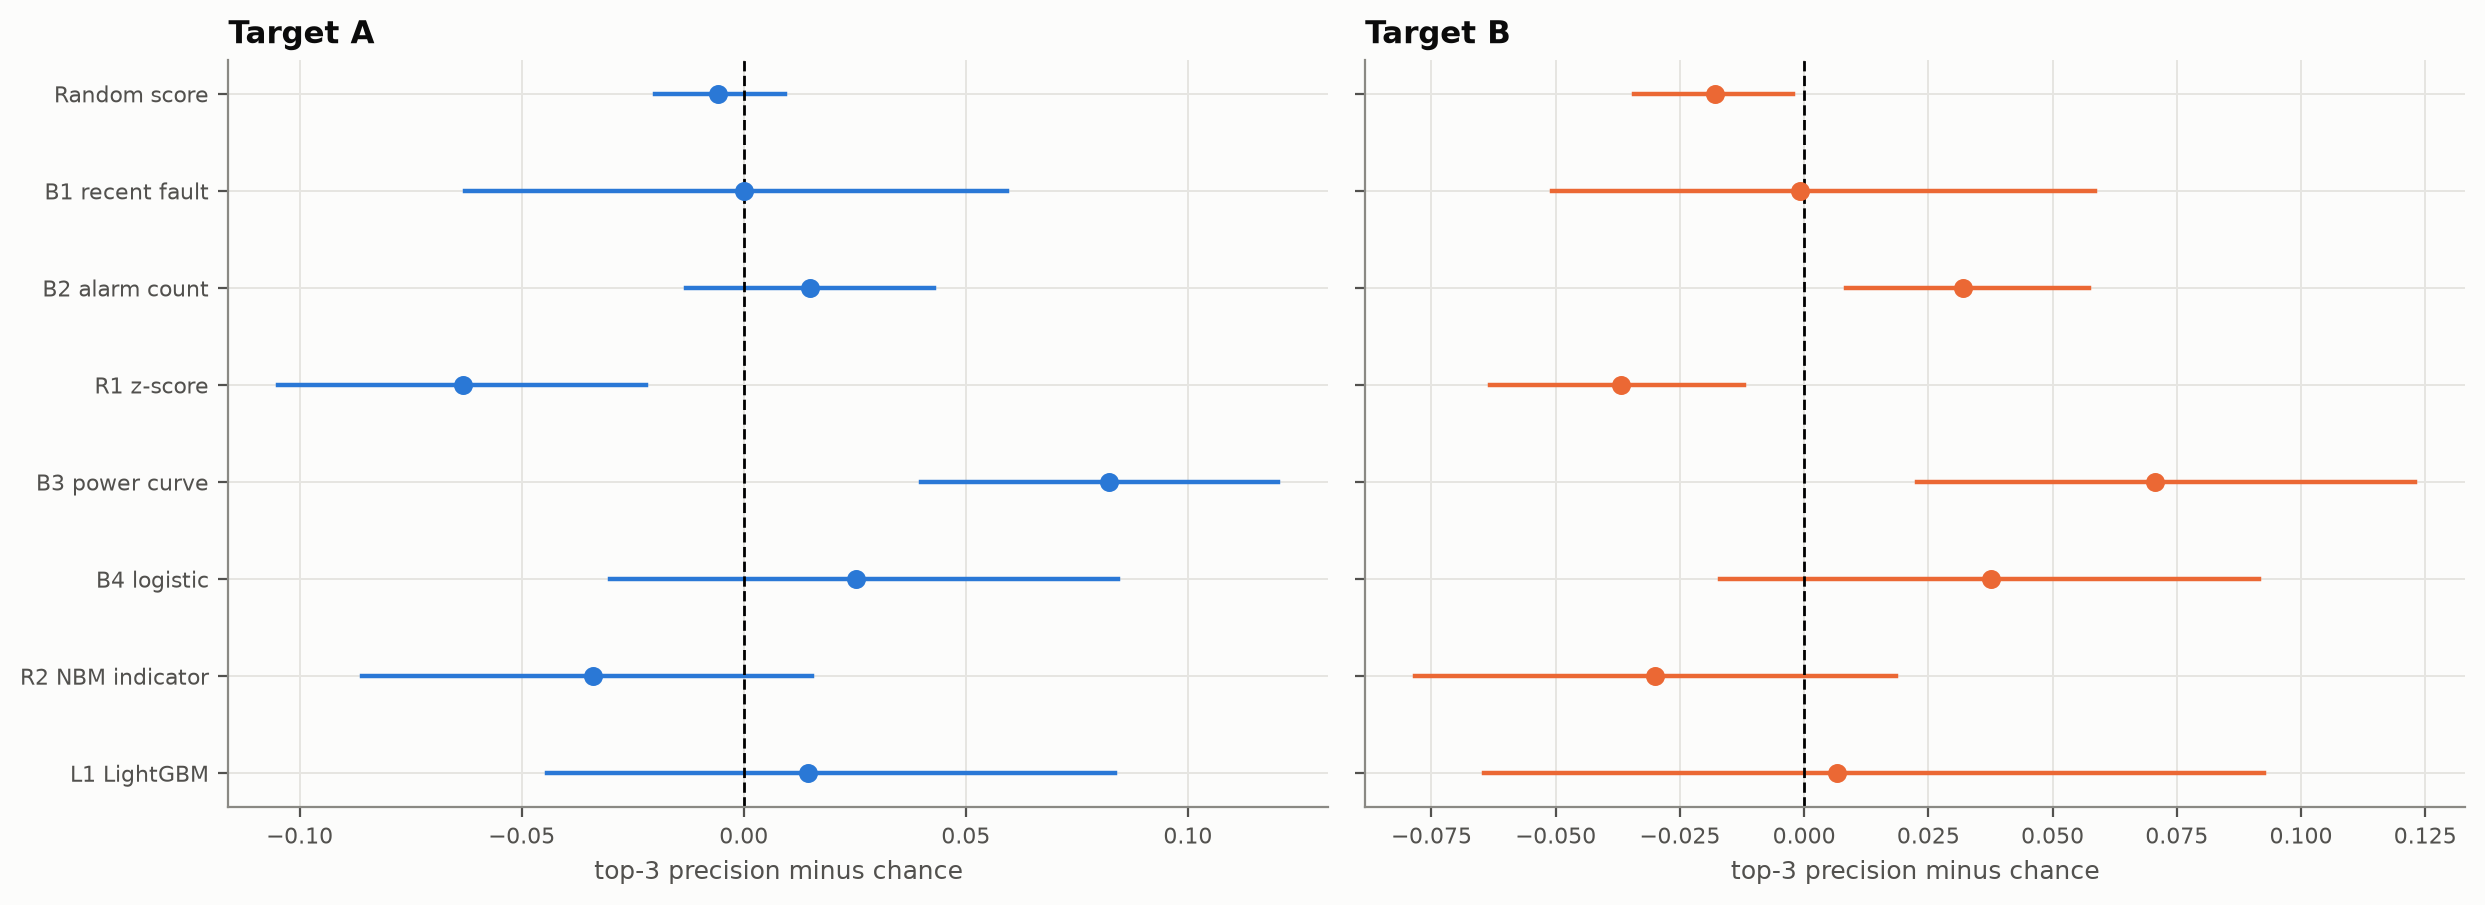
\includegraphics[width=\linewidth]{08_exploratory/F39_turbine_ranking.png}
	\caption{Top-3 ranking against chance on the validation years (F39). The power-curve baseline B3 is above chance for both targets; the z-score R1 is below it.}
	\label{fig:ranking}
	\end{figure}

	\paragraph{Round 3: ranking the features and pruning the least useful.} Using only the labelled training rows, the columns were ranked three ways (LightGBM gain averaged over fits that each leave one training year out; whether a column's own AUC lies on the same side of 0.5 in every training year; and the first ranking with near-duplicate columns skipped), the top 10, 25, 50 or 100 were kept, and the two main models were refitted on the raw and self-baseline features, with the ranking recomputed inside each fit. Compared with the same model on all columns, the 96 pruned versions changed validation PR-AUC by between $-0.051$ and $+0.027$ (average $-0.002$) and lowered the check on training years in 79 of 96 (Figure~\ref{fig:pruning}); no interval excluded the random-score value, and refitting with one whole group of sensors or alarm counts removed changed the score by between $-0.030$ and $+0.021$. Keeping 50 or 100 columns cost nothing measurable, so the models can be simplified, but no subset gave a result beyond the margin of error. About a quarter to a third of the gain sits outside the top 50 columns, the pressure and hub sensors and days since the last fault dominate the top of the ranking, and only 31 (target A) and 85 (target B) columns point the same way in every training year; for target B the most stable are ambient and nacelle temperatures, which follow the season and may reflect weather rather than turbine wear. The two rankings disagree (only 5 of the top 25 columns by gain are also in the top 25 by year-stability), and the year-stability filter did worse than the gain ranking.

	\begin{figure}[htbp]
	\centering
	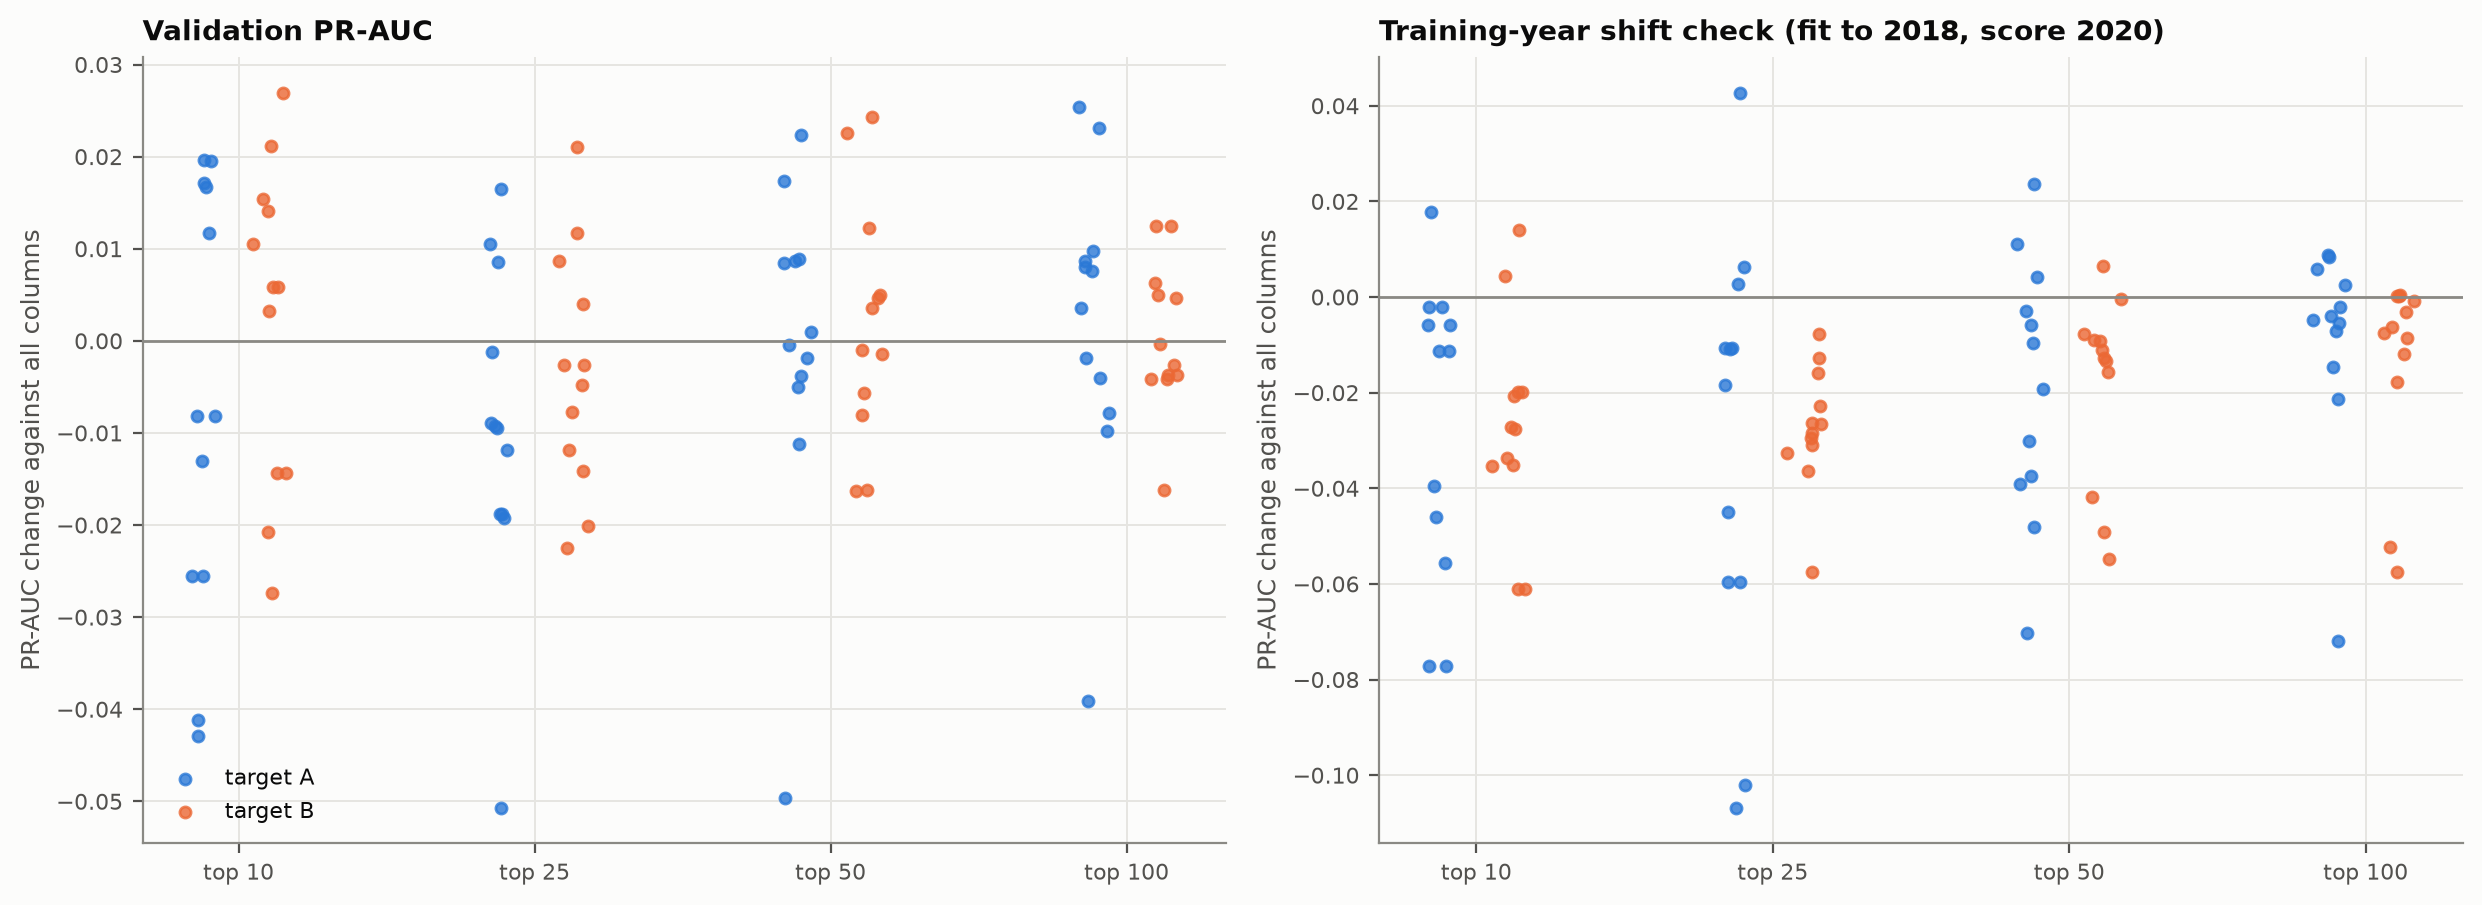
\includegraphics[width=\linewidth]{08_exploratory/F37_feature_pruning.png}
	\caption{Pruning the features (F37): the change in PR-AUC of each pruned configuration against the same model with all columns, on validation (left) and on the training-year check (right). Blue: target A; orange: target B.}
	\label{fig:pruning}
	\end{figure}

	\paragraph{Round 4: other label definitions.}\label{sec:labelsens} Because every model sat at the random-score floor, we asked whether the labels were the bottleneck. The labels were rebuilt in memory (the frozen files were only read, to check that the reference variant reproduces them exactly) with the positive window set to 7, 14 or 30 days; with a fault day defined as at least 4, 8 or 12 hours of recorded fault time (target A) or a stop lasting 3, 6 or 12 hours (target B); and, for target B, with or without the stops that began while a low-wind, high-wind or icing alarm was active, giving 9 and 18 variants. The seven models were rerun unchanged and each variant was compared with its own random-score floor (Table~\ref{tab:labelsens}, Figure~\ref{fig:labelsens}). More specific labels raised the typical score a little over the floor (median ratio 1.05 to 1.18 for target A and 1.12 to 1.25 for target B as the severity rose, and 1.26 against 1.11 for target B without weather stops), but the learned models did not benefit: LightGBM was above the floor in 1 of 27 variants and the logistic model in none. The variants above the floor came from simple rules, mainly the power-curve baseline B3 (above chance in the turbine ranking in 16 of 18 variants of target B and 4 of 9 of target A) and the recent-fault rule, which mostly reflects that a turbine that recently faulted tends to fault again. The z-score model ranked turbines worse than chance in 8 of 18 variants of target B. The variants overlap heavily (the same days, nested definitions) and 189 intervals were examined, so the 37 above the floor overstate the evidence; the conclusion is that the labels are not the main bottleneck for the learned models, and that B3's ranking advantage survives most label definitions.

	\begin{table}[htbp]
	\centering
	\scriptsize
	\resizebox{\linewidth}{!}{\begin{tabular}{@{}lrrrrrrrr@{}}
\toprule
 & \multicolumn{4}{c}{Target A (9 variants)} & \multicolumn{4}{c}{Target B (18 variants)} \\
\cmidrule(lr){2-5}\cmidrule(lr){6-9}
Model & PR-AUC above floor & Median lift & Ranking above chance & Ranking below chance & PR-AUC above floor & Median lift & Ranking above chance & Ranking below chance \\
\midrule
B1 recent fault & 3 & 1.27 & 0 & 0 & 9 & 1.53 & 11 & 0 \\
B2 alarm count & 2 & 1.21 & 0 & 0 & 0 & 0.99 & 2 & 0 \\
R1 z-score & 3 & 1.10 & 0 & 1 & 6 & 1.18 & 0 & 8 \\
B3 power curve & 0 & 1.00 & 4 & 0 & 11 & 1.67 & 16 & 0 \\
B4 logistic & 0 & 0.99 & 0 & 0 & 0 & 1.07 & 3 & 0 \\
R2 NBM indicator & 0 & 1.03 & 0 & 0 & 2 & 1.11 & 0 & 0 \\
L1 LightGBM & 0 & 1.05 & 2 & 0 & 1 & 1.15 & 6 & 0 \\
\bottomrule
\end{tabular}
}
	\caption{Round 4, label sensitivity on the validation years. For each model: the number of label variants whose PR-AUC interval lies above that variant's random-score floor, the median ratio of PR-AUC to the floor, and the number of variants in which the daily top-3 ranking is above or below chance (95\% interval excludes zero).}
	\label{tab:labelsens}
	\end{table}

	\begin{figure}[htbp]
	\centering
	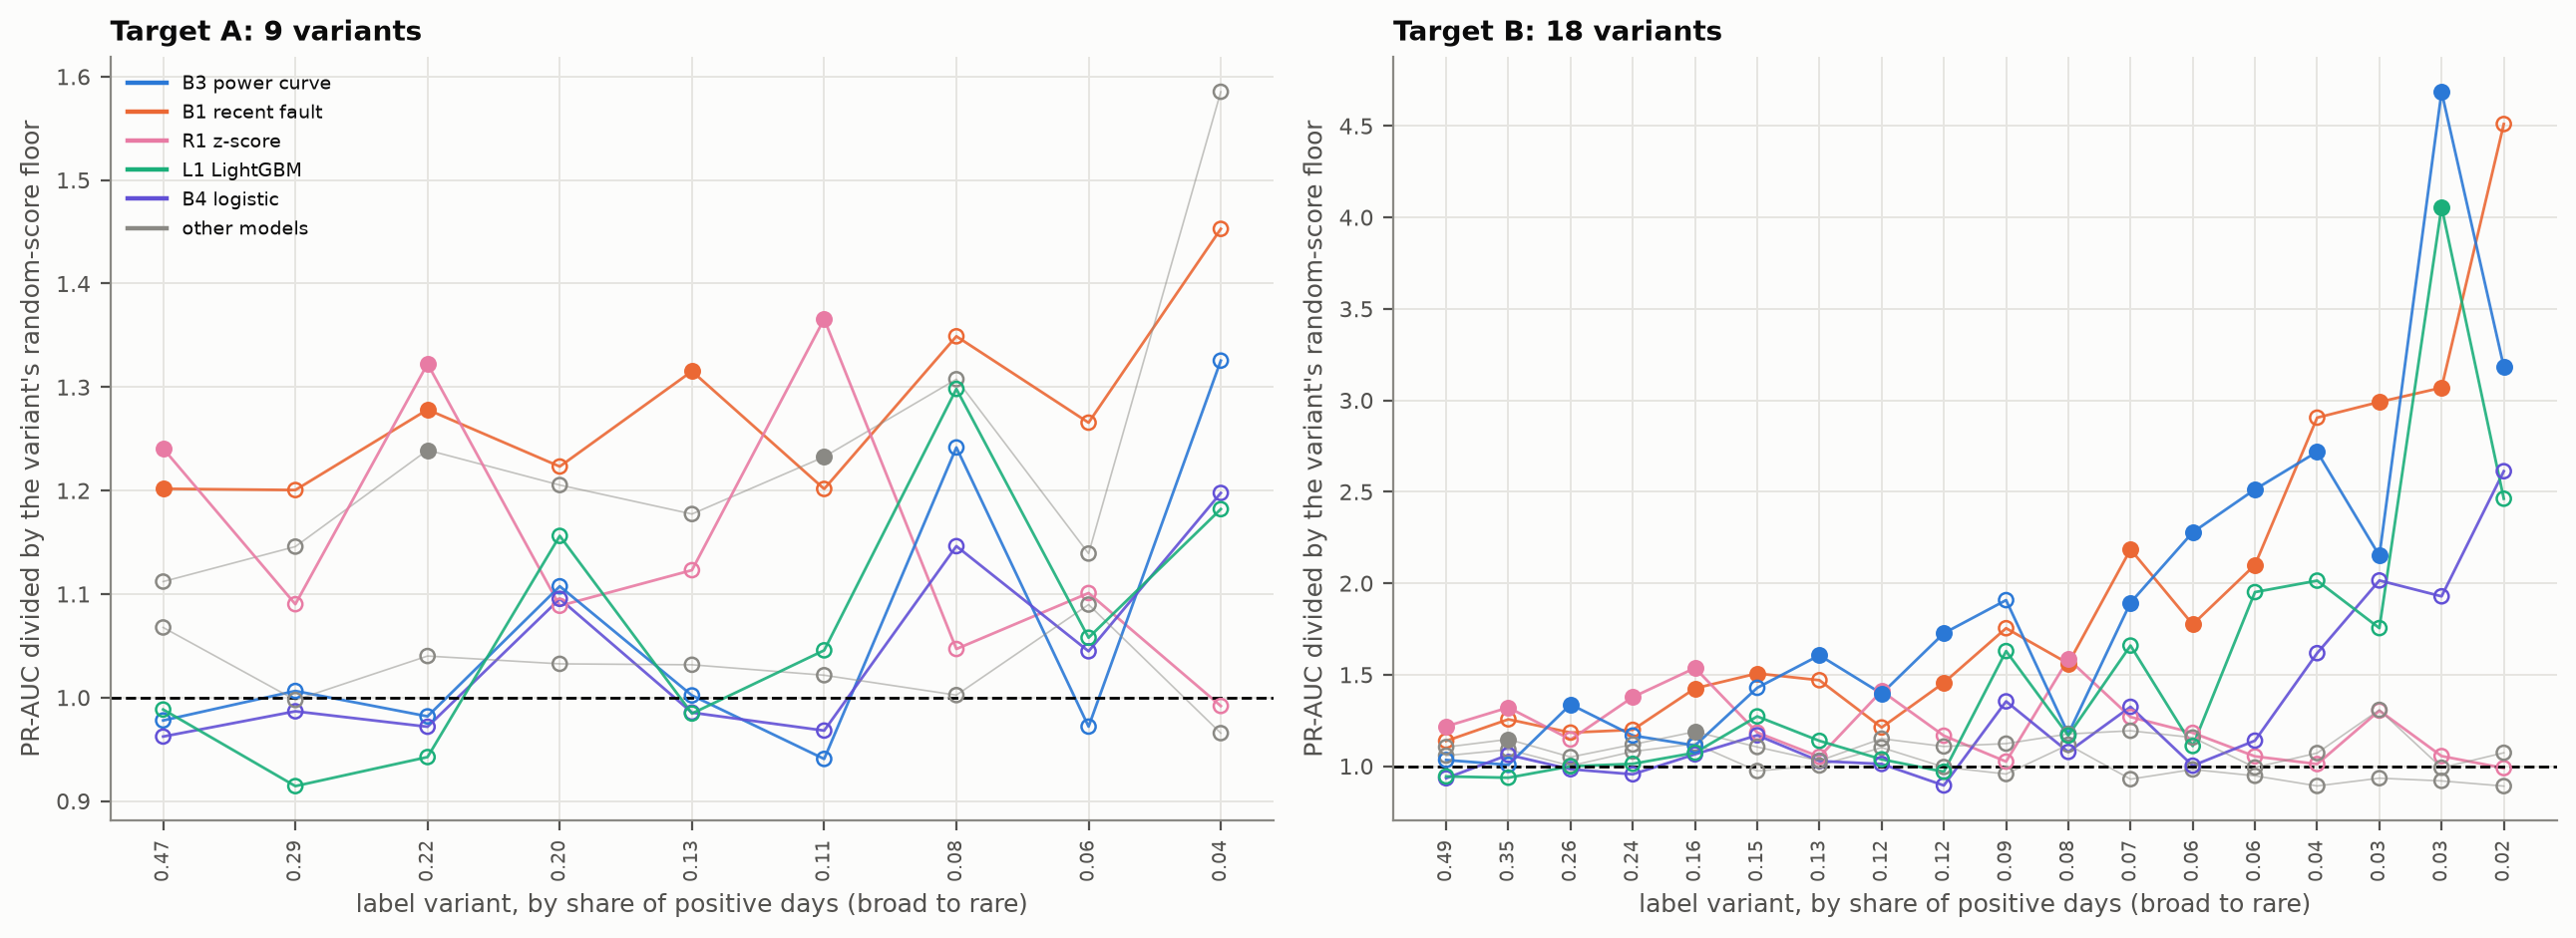
\includegraphics[width=\linewidth]{08_exploratory/F38_label_sensitivity.png}
	\caption{Label sensitivity (F38): PR-AUC divided by each variant's own random-score floor, with variants ordered from the broadest (left) to the rarest (right) label. Filled markers have intervals above the floor. A ratio grows when the floor is small, so it must be read with the markers.}
	\label{fig:labelsens}
	\end{figure}

	\paragraph{Taken together.} The four rounds point the same way. Changing the inputs (fleet-relative, self-baseline, pruned) or the labels moved validation scores by a few hundredths in both directions without moving any learned model beyond the random-score margin; a model that is simple can be as good as a complex one; and the only consistent pattern is that a rotor-speed-against-wind-speed curve ranks turbines above chance on the tuning years. None of this was tested on the test years.

	%===========================================================
	\section{Limitations and Shortcomings}\label{sec:limits}\label{sec:issue}
	We list what limits the conclusions, how we dealt with each and how far that helped. Items are grouped by where in the pipeline they arise.

	\subsection{Data}
	\begin{itemize}
		\item \textbf{Missing tables.} Active power and error time were not in our files, so the power-curve baseline uses rotor speed against wind speed and the meaning of \texttt{TimeErr} is inferred. We defined a second target from the 10-minute data and reported both, but neither is a confirmed failure.
		\item \textbf{A missing year and outage months.} 2019 has no temperature or pressure tables in our copy and is not used (a later copy of the raw files contained 2019, but we kept the split fixed); three outage months and four turbine-years with a suspect wind sensor are flagged, not dropped. Training therefore has four years, one of them (2020) separated from the others by the gap.
		\item \textbf{Sensors and levels change over time.} Some sensors exist only in some years (Figure~\ref{fig:sensors}), temperature and pressure levels drift between years, a step change occurs in the secondary anemometer, and the alarm counts of two routine codes roughly halve in 2022. We chose columns and imputation on training years only, used the primary wind channel, and made the normal-behaviour residuals relative to the fleet.
		\item \textbf{An unusual turbine.} Turbine 2304515 is positive on 97\% of its validation days; we report validation results with and without it, and left it out of the normal-behaviour fit.
		\item \textbf{One farm, one turbine model.} Nothing here shows that a model transfers to another site; the open dataset has no measured power, confirmed failure or maintenance records, and alarm descriptions exist for only 12 codes.
	\end{itemize}

	\subsection{Labels}
	\begin{itemize}
		\item \textbf{Inferred episodes, not failures.} ``Fault'' means recorded fault time or a rotor stop of three hours, which also includes weather and grid events. Round 4 tested stricter and weather-free variants, and they did not help the learned models, but they remain proxies.
		\item \textbf{About half of the days are positive.} With a 30-day window a random score already reaches recall of 0.76 to 0.84 at the budget, so the headline recall at one false alarm per turbine-month is uninformative. We report PR-AUC and recall against the random-score floor for every model and label variant. The overlap of the 30-day windows also means neighbouring labelled days are strongly dependent.
		\item \textbf{The targets are related.} About three quarters of the episodes of one have an episode of the other nearby, so reporting both is a robustness check and not two independent replications; B1 also uses target A's history for both targets.
	\end{itemize}

	\subsection{Evaluation}
    The evaluation review (D-069) checks consistency of the 48 published runner rows,
    frozen threshold carryover and random floors. Independent reproduction of current
    metrics and intervals remains pending transfer of the original saved scores;
    no model was refitted or rescored for that review.

    False-alert days and missed inferred episodes are workload proxies, not inspection
    visits or prevented failures. Consecutive alerts are not consolidated, and unlabelled
    days do not enter this burden estimate. The dataset supplies no verified visit cost,
    failure cost or intervention benefit, so no currency saving or economic optimum is claimed.

	\begin{itemize}
		\item \textbf{Validation did not predict test.} The model ranking changed between validation and test, the best validation model (R1) fell to the random level, and the alert threshold chosen on validation did not hold the false-alarm rate on test (0.25 to 2.5 per turbine-month against a budget of one). We scored the test years once and report both; this also means we could not tune after seeing test.
		\item \textbf{Short validation, long test.} Two validation years are a thin basis for choosing settings, and the test years span more than three years of further drift.
		\item \textbf{Intervals are partial.} They resample whole turbines with the threshold fixed, so they ignore the uncertainty of choosing the model and threshold and the dependence between turbines in the same weather. They are probably narrower than the true uncertainty.
		\item \textbf{Multiple looks.} About 390 model runs and several hundred ranking intervals were examined on the validation years, so some will look better than random by luck; B2's variant and B4's regularisation were also chosen on validation, so those values are optimistic. We pre-registered each round and report all configurations, but we cannot remove this bias, which is why exploratory results are labelled leads.
		\item \textbf{Scored rows.} Four labelled test days of target A have no features and are not scored, and nine target B episodes are not evaluated. \tbc{Confirm the reason.}
	\end{itemize}

	\subsection{Modelling}
	\begin{itemize}
		\item \textbf{Overfitting to year-specific levels.} LightGBM reached a PR-AUC of 0.94 in-sample against about 0.45 on held-out years. Fleet-relative and self-baseline features, pruning and small models did not close this gap.
		\item \textbf{A weak normal-behaviour model.} The ridge models fit some sensors poorly (R-squared 0.11 for hydraulic oil), the indicator is only slightly higher before episodes, and it drifts between years unless made relative to the fleet.
		\item \textbf{Settings fixed on the 30-day label.} The LightGBM grid was small (six settings) and the frozen settings were not retuned for other horizons or severities, so the shorter-horizon variants are partly a mismatch for them.
		\item \textbf{Methods not tried.} We did not fit sequence models, joint models of all sensors (for example autoencoders or principal-component reconstruction error), per-turbine anomaly detectors, or survival models, and we did not run the upgrade analysis. Section~\ref{sec:disc} lists them as future work.
		\item \textbf{Explanations are attribution.} SHAP ranks inputs for a model that has no demonstrated skill, so a stable ranking says nothing about causes.
	\end{itemize}

	\subsection{Process}
	\begin{itemize}
		\item \textbf{Unverified items.} The citations, the dataset version, the temperature-field count, the publishers' stated intended use, the upgrade names and dates, the hardware and the ethics review are still open (marked in red), and the report could not be compiled in the environment where it was written, so figures, tables and cross-references have been checked only for existence.
	\end{itemize}

	%===========================================================
	\section{Discussion: Recommendations, Stakeholders, Impact and Ethics}\label{sec:disc}

	\subsection{What the Findings Mean}
	With these data and labels, none of the models shows a gain over a random score on the test years that survives the uncertainty of the estimate, so the models cannot yet tell an operator which turbine to inspect first. The learned models were modestly ahead of the simple rules in point estimates, but not beyond the margin of error. This is a limit of the evidence, not proof that prediction is impossible: the target is broad (a 30-day window with about half of days positive), the labels are inferred episodes and not confirmed failures, and the sensors drift between years. The follow-up rounds say where not to look further (more feature engineering and label tweaking did not help the learned models) and where one might (the rotor-speed curve ranks turbines above chance on the tuning years). The value of any warning still depends on whether its lead time can be acted on: days allow a technician visit and parts to be scheduled during low wind, when lost production is smallest.

	\subsection{Recommendations}
	\begin{enumerate}
		\item \textbf{Do not deploy these models for operations.} None beats the random score on the test years; keep existing protection and inspection routines.
		\item \textbf{If a model is used later, use it as decision support, not control,} to rank turbines for human review, with turbine protection as the final safeguard.
		\item \textbf{Set the threshold from costs, on recent data.} Choose $\tau$ to minimise $C_{\text{FP}}N_{\text{FP}} + C_{\text{FN}}N_{\text{FN}}$ (unnecessary inspection vs.\ unplanned stop). Our validation threshold did not carry to later years, so it should be re-chosen on recent data and monitored. Such costs were unavailable, so this is a future decision framework rather than an estimated optimum.
		\item \textbf{Retrain and recheck after upgrades and across years.} The data period includes the AeroUp and TuneUp upgrades \cite{hot_dataset_v1}; we could not test their effect, and sensor drift across years was visible, so models should be recalibrated and monitored for drift. \tbc{Check the upgrade names and dates against the dataset.}
		\item \textbf{Track the false-warning rate as a key performance indicator,} since frequent false warnings recreate the alarm overload of \cite{qiu2012}.
		\item \textbf{Obtain better labels first:} confirmed failure and maintenance records, active power and the documented error time, which would replace the inferred episodes.
	\end{enumerate}

	\subsection{Stakeholders and Impact}
	\begin{table}[htbp]
	\centering
	\small
	\begin{tabularx}{\linewidth}{@{}lX@{}}
	\toprule
	\textbf{Stakeholder} & \textbf{Impact of the system} \\
	\midrule
	Owners/investors (e.g.\ TRIG) & Potential for fewer unplanned stops and lower O\&M spend if a model is later shown to work; no benefit demonstrated yet. \\
	Operators (e.g.\ RES) & Prioritised work lists in future; a real risk of alert fatigue if false warnings are frequent, as our alert rates show. \\
	Technicians & More planned work in good weather and fewer emergency call-outs if warnings prove reliable; they need to trust warnings. \\
	Manufacturer / service provider & Evidence for root-cause analysis; overlap with proprietary monitoring. \\
	Grid and consumers & Slightly more predictable output if unplanned stops fall. \\
	Community and environment & Fewer crane and vehicle movements; more renewable energy delivered. \\
	\bottomrule
	\end{tabularx}
	\caption{Stakeholders of a SCADA-based fault-prediction system.}
	\label{tab:stake}
	\end{table}

	As O\&M is a large share of wind LCOE \cite{irena2012}, even modest cuts in unplanned downtime would lower energy costs, while planned maintenance reduces time spent working at height under pressure or in poor weather (Table~\ref{tab:stake}). Our results show that this benefit is not yet established.

	\subsection{Ethical Considerations}
	\begin{itemize}
		\item \textbf{Over-reliance:} the gravest risk is a false negative that a trusting operator fails to catch. The models must supplement, not replace, existing protection and inspections, and our results show that they do not yet beat chance.
		\item \textbf{Alert fatigue:} false positives waste technician time and erode trust, so the threshold is an ethical choice to be set transparently with those who act on it. On the test years our validation thresholds gave between 0.25 and 2.5 false alarms per turbine-month.
		\item \textbf{Accountability and honest reporting:} we report a weak result as weak, with intervals, we state how many configurations were tried, and we explain predictions as model attribution and not as causes, so that engineers can see why a warning fired and override it.
		\item \textbf{Generalisability:} trained on one farm, turbine type and climate, the model may fail silently elsewhere and must be revalidated before transfer.
		\item \textbf{Data use:} the CC-BY-4.0 licence requires attribution to TRIG and RES. \tbc{That the publishers removed SCADA user identifiers \cite{hot_dataset_v1} and the exact citation text still need to be checked against the record page.} Commercial use on proprietary data would raise data-ownership questions.
		\item \textbf{Limits of the open data:} there are no measured power, confirmed failure or maintenance records, and alarm descriptions exist for only 12 codes. ``Fault'' and ``degradation'' are inferred. \tbc{Ethics review (Cyrus): confirm and extend this section.}
	\end{itemize}

	\subsection{Future Work}
	In order of expected value:
	\begin{enumerate}
		\item \textbf{Better labels.} Obtain confirmed failure and maintenance records and the missing power and error-time tables, and redefine the targets from them. This addresses the largest limitation directly.
		\item \textbf{Confirm the power-curve lead on data not used here.} Check whether the rotor-speed-against-wind-speed baseline keeps its ranking advantage on fresh or external data under a pre-registered protocol (for example the CARE benchmark \cite{gueck2024}, which has labelled fault logbooks), rather than looking again at the test years.
		\item \textbf{Joint and unsupervised models.} Models that learn the joint behaviour of many sensors on healthy days, such as principal-component or autoencoder reconstruction error, and per-turbine anomaly detectors such as isolation forests, are widely used for turbine condition monitoring \tbc{add and verify citations before submission} and extend our indicator and the power-curve lead without needing labels.
		\item \textbf{Timing-aware targets.} Time-to-event or survival formulations, and episode-onset-only targets, as a separate pre-registered study; we examined the horizon only through label variants.
		\item \textbf{Operational set-up.} Re-estimate the alert threshold on recent data and test how stable it is; add the upgrade analysis once installation dates are available; adopt an earliness-weighted score such as the CARE score \cite{gueck2024}; exploit the $\sim$1\,Hz data added in v2.1.0 \cite{hot_dataset_v2} with sequence models; and run a shadow trial logging predictions alongside live operations to measure real lead time.
	\end{enumerate}

	\section{Conclusions}
	We asked whether routine SCADA data can warn of a fault or long stoppage in a wind turbine 30 days ahead. On 21 turbines and about ten years of data, with two related fault definitions, the answer from this work is not yet. Three findings stand out:
	\begin{enumerate}
		\item \textbf{No model beats the random score on the test years.} Every 95\% interval for PR-AUC contains the random-score value (0.450 for A, 0.506 for B); the best point estimates are 0.493 (LightGBM, A) and 0.563 (logistic regression, B), about 0.04 above the best simple rule.
		\item \textbf{The validation ranking and threshold did not carry over.} The z-score model that led on validation (0.577 and 0.588) fell to the random level on test (0.448 and 0.499), and its alerts reached about 2.1 false alarms per turbine-month against a budget of one.
		\item \textbf{The normal-behaviour indicator and the explanations are stable but weak.} The indicator drifts between years unless made relative to the fleet and is only slightly higher before episodes; the model's ranking of inputs is stable across turbines but describes a model without demonstrated skill.
	\end{enumerate}
	Four exploratory rounds on the validation years (about 390 runs) found that fleet-relative and self-baseline features, pruning to 50--100 inputs, and 27 alternative label definitions did not lift the learned models beyond the margin of error, and that the one consistent signal is a power-curve baseline that ranks turbines above chance; none was tested on the test years, and they are leads for future work. Of the objectives, O1 (indicator) and O4 (explanation) were built and found weak, O2 (prediction) was built and evaluated honestly but does not beat chance, and O3 (robustness) was met for unseen turbines and missing sensor groups on the validation years, while the upgrade analysis was not run. Our key recommendation is to not deploy these models and to improve the labels before repeating the study; the first next step is to obtain confirmed failure and maintenance records, and the second is to test the power-curve lead on data we have not looked at.

	%===========================================================
	\bibliographystyle{ieeetr}
	\bibliography{refs}

\end{document}
